%%%%%%%%%%%%%%%%%%%%%%%%%%%%%%%%%%%%%%%%%%%%%%%%%%%%%%%%%%%%%%%%%%%%%%%%%%%%%%%%
%2345678901234567890123456789012345678901234567890123456789012345678901234567890
%        1         2         3         4         5         6         7         8

\documentclass[letterpaper, 10 pt, conference]{ieeeconf}  % Comment this line out
                                                          % if you need a4paper
%\documentclass[a4paper, 10pt, conference]{ieeeconf}      % Use this line for a4
                                                          % paper

\IEEEoverridecommandlockouts                              % This command is only
                                                          % needed if you want to
                                                          % use the \thanks command
\overrideIEEEmargins
% See the \addtolength command later in the file to balance the column lengths
% on the last page of the document



% The following packages can be found on http:\\www.ctan.org
%\usepackage{graphics} % for pdf, bitmapped graphics files
%\usepackage{epsfig} % for postscript graphics files
%\usepackage{mathptmx} % assumes new font selection scheme installed
%\usepackage{times} % assumes new font selection scheme installed
\usepackage{caption}
\usepackage{subfig}
\usepackage{amsmath} % assumes amsmath package installed
\usepackage{bm}
\usepackage{amssymb}  % assumes amsmath package installed
\usepackage{boldline}
\usepackage{array,multirow}
\usepackage{hyperref}
\usepackage{color}
\usepackage{graphicx}
\graphicspath{ {images/} }
\definecolor{light-gray}{gray}{0.95}
\newcommand{\code}[1]{\colorbox{light-gray}{\texttt{#1}}}
\DeclareMathOperator*{\argmax}{arg\,max}
\DeclareMathOperator*{\maxU}{max}
\usepackage{makecell}
\usepackage{bbm}
\usepackage[table,xcdraw]{xcolor}
\usepackage[flushleft]{threeparttable}
\usepackage[utf8]{inputenc}
\usepackage{xfrac}
\usepackage{capt-of}
\usepackage{algorithm}
\usepackage[noend]{algpseudocode}


\title{
A Closer Look At The Convergence of Adam and AMSGrad \\
\large Track 3: A Reproducibility Study, Concerning \emph{On the Convergence Of Adam and Beyond} \\
by Sashank, Kale, Kumar; 2018.
}

\author{ 
	\parbox{2 in}{\centering Tamir Bennatan
         {\tt\small tamir.bennatan@mail.mcgill.ca\\}
         {\tt\small 260614526}}
         \hspace*{ 0.3 in}
         \parbox{2 in}{\centering L\'ea Collin
         {\tt\small lea.collin@mail.mcgill.ca\\}
         {\tt\small 260618407}}
         \hspace*{0.3 in}
         \parbox{2 in}{\centering Emmanuel Ng Cheng Hin
         {\tt\small emmanuel.ngchenghin@mail.mcgill.ca\\}
         {\tt\small 260615964}}
}



\begin{document}



\maketitle
\thispagestyle{empty}
\pagestyle{empty}

%%%%%%%%%%%%%%%%%%%%%%%%%%%%%%%%%%%%%%%%%%%%%%%%%%%%%%%%%%%%%%%%%%%%%%%%%%%%%%%%
\begin{abstract}
In this study, we assess the reproducibility of the results reported in the paper \emph{On the Convergence of Adam and Beyond} (Sashank, Kale \$ Kumar; 2018). The authors of this paper discuss issues with a popular variant of stochastic gradient descent called \emph{Adam}, and propose an improved algorithm, \emph{AMSGrad}. In this paper, we recreate four experiments described by the authors - one using a synthetic dataset, and three using the MNIST and CIFAR-10 datasets. We report results that are less conclusive than those reported by the authors, and discuss details that were omitted from the original paper that hinder reproducibility of the authors' results.
\end{abstract}

%%%%%%%%%%%%%%%%%%%%%%%%%%%%%%%%%%%%%%%%%%%%%%%%%%%%%%%%%%%%%%%%%%%%%%%%%%%%%%%%
\section{INTRODUCTION}

Amongst the deep learning community, Stochastic Gradient Descent (SGD) is the predominant method of training deep neural networks. As researchers and practitioners continue to experiment with large networks with parameter spaces reaching hundreds of millions of dimensions, it has become increasingly important in recent decades to optimize SGD, so that it may train large networks faster and more effectively. 

One such optimization to SGD is \emph{Adam} (Kingma, Ba; 2015). Inspired by previous variants of SGD which  apply time varying learning rates and momentum terms such as AdaGrad (Duchi et al.,
2011) and RMSProp (Tieleman \& Hinton, 2012), Adam adjusts the learning rates and momentum terms associated with each parameter of a network using exponential moving averages. In recent years, Adam has been shown to be effective in many deep learning settings, and is considered a state of the art technique. 

In the paper \emph{On the Convergence of Adam and Beyond}, authors Sashank, Kale and Kumar (2018) present a defect in the Adam method. Since Adam uses exponential moving averages of squared past gradients, each gradient's influence on future parameter updates drops off quickly - effectively limiting the reliance of parameter updates to a small set of recent gradients. The authors show that because of this property, Adam will fail to converge in convex optimization problems where large, informative gradients occur infrequently. 

The authors propose a new optimization scheme - \emph{AMSGrad}, which aims to remedy this issue. To demonstrate that AMSGrad performs better than Adam, they devise a synthetic convex optimization problem, and show that AMSGrad converges to the optimal solution, while Adam converges to a highly suboptimal solution. They then train neural networks on the widely used MNIST and CIFAR-10 datasets using the Adam and AMSGrad optimizers, and show that the networks trained with AMSGrad converge to a lower loss than those trained with Adam. 

In this paper, we recreate the experiments described in the paper\footnote{We refer to \emph{On the Convergence of Adam and Beyond} as simply \emph{``the paper"}, the authors of this paper as ``\emph{the authors}" throughout.} and aim to reproduce the authors' results. We compare our results with those of the authors, and discuss the challenges in recreating the experiments described in this paper. Finally, we present a brief sensitivity analysis, to gauge the variability in our findings.

\section{AMSGrad: LONG TERM MEMORY OF GRADIENTS}

Adaptive optimization procedures such as Adam yield different effective learning rates for each of the different parameters of a model.

If we consider a model with a single parameter, $\theta$, then Adam uses the following update step to optimize the function $f_{t}(x)$ at time $t$:

\begin{algorithm}
\caption{Adam Update Rule}\label{Adam-update}
\begin{algorithmic}[1]
\State $g_t = \nabla_{\theta}f_t(x_t)$
\State $m_t = \beta_{1t}m_{t-1} + (1 - \beta_{1t})g_t$ 
\Comment{Adaptive Momentum}
\State $v_t = \beta_2{v_{t-1}} + (1-\beta_2)g_t^2$
\Comment{Adaptive learning rate}
\State $\theta_{t + 1} := \theta_t - \alpha{v_t}$
\end{algorithmic}
\end{algorithm}
Where $\alpha$ is the learning rate, and $(\beta_1, \beta_2)$ are hyperparameters chosen in the range $(0,1)$.

The exponential moving average terms on lines 2 and 3 of Alg. 1 reduce the reliance of each update on past gradients geometrically. The authors show that because of this property, the effective learning rate of each parameter is not guaranteed to be non-decreasing, which causes convergence issues in particular settings. 

To account for this, the authors modify Adam to ``remember" large gradients from further in the past:

\begin{algorithm}
\caption{AMSGrad Update Rule}\label{Adam-update}
\begin{algorithmic}[1]
\State $g_t = \nabla_{\theta}f_t(x_t)$
\State $m_t = \beta_{1t}m_{t-1} + (1 - \beta_{1t})g_t$ 
\State $v_t = \beta_2{v_{t-1}} + (1-\beta_2)g_t^2$
\State $\hat{v_t} = max(\hat{v}_{t-1}, v_t)$
\Comment{Propagate large updates}
\State $\theta_{t + 1} := \theta_t - \alpha{\hat{v_t}}$
\end{algorithmic}
\end{algorithm}

Line 4 of Alg. 2 enables AMSGrad to propagate the large gradients into the future, which increases their effect on future updates. The authors show that after making this adjustment, AMSGrad guarantees non-increasing effective learning rates, and favorable convergence behavior.

To illustrate this, the authors propose a simple convex function on the domain $x \in [-1,1]$:
\[
    f_{t}(x) = 
    \begin{cases}
     	Cx, \hspace{5mm} \text{for } t \text{ mod 3 = 1} \\
        -x, \hspace{5mm} \text{otherwise}
    \end{cases}
\]
for $C>2$. The minimum value of $f$ is achieved at $x=-1$. However, the authors show that Adam converges to the suboptimal solution of $x = 1$, due to the fact that the large gradients with magnitude $C$ are only observed once every three time steps. The influence of this large gradient $C$ disappears too quickly to counteract the gradients of $-1$, which move the algorithm in the wrong direction. AMSGrad, on the other hand, is designed to account for these settings, and minimizes this function without difficulty.

\section{Experiments}


The authors ran several experiments to compare the performance of Adam and AMSGrad. In this section, we 
describe these experiments, and their reported results. 

\subsection{Synthetic Experiments}

The authors construct two convex functions on the domain $x \in [-1,1]$, designed to highlight Adam's shortcomings:

\[
    f_{t}(x) = 
    \begin{cases}
     	1010x, \hspace{5mm} \text{for } t \text{ mod 101 = 1} \\
        -10x, \hspace{5mm} \text{otherwise}
    \end{cases}
\]
where $t$ is the time step at which the function is evaluated, and:

\[
    f_{t}(x) = 
    \begin{cases}
     	1010x, \hspace{5mm} \text{with probability 0.01}\\
        -10x, \hspace{5mm} \text{otherwise}
    \end{cases}
\]

Both functions reach a global minimum at $x = -1$. The first is referred to as the ``online setting", and the second as the ``stochastic setting."

The authors use Adam and AMSGrad to minimize both functions, and compare the convergence behavior of each optimizer. The authors fix the values of  $\beta_{1}$ and $\beta_{2}$ at 0.9 and 0.99, respectively, and perform a grid search to find a learning rate $\alpha$ which yields good convergence for both optimizers. 

\subsection{Logistic Regression on MNIST}

The authors then investigated the performance of the each optimizer in training a logistic regression classifier. They used the MNIST dataset, which contains 70,000 28x28 images of handwritten digits, labeled as one of 10 classes. The authors decrease the learning rate over time, where the learning rate $\alpha_t$ at time $t$ is defined as $\alpha / \sqrt{t}$ for a fixed $\alpha$. The authors train using minibatches of size 128, and fix  $\beta_{1}$ to be 0.9. They then perform a grid search to select a value for $\beta_2$ in the range $(0.99, 0.999)$, and to select a value for $\alpha$, for which no range of values is provided.

\subsection{Feedforward Neural Network on MNIST}

The authors trained a feedforward neural network with one hidden layer on the MNIST dataset as well. The hidden layer consists of 100 neurons, and uses the ReLU nonlinearity. The authors fix $\beta_{1} = 0.9$, and use a grid search to select $\beta_{2}$ from the range $(0.99, 0.999)$, and to select a value for $\alpha$, for which no range of values is provided. These hyperparameters were then chosen based on which value yielded the lowest validation loss for each optimizer. 

\subsection{Convolutional Neural Network on CIFAR-10}

Finally, the authors experiment with a larger convolutional neural network (CNN), designed to classify images in the CIFAR-10 dataset. CIFAR-10 consists of 60,000  32x32 images, labeled as one of 10 classes.

The authors specify the architecture that they used (named \emph{CifarNet}), which consists of two convolutional layers, max-pooling and batch-normalization layers, and two fully connected layers (see appendix 1 for a detailed specification of the architecture.)

The authors trained CifarNet using a minibatch of size 128 using each of the two optimizers.The authors fix $\beta_{1} = 0.9$, and perform a grid search to select $\beta_{2}$ from the range $(0.99, 0.999)$, and to select a value for $\alpha$, for which no range of values is provided.

\subsection{Results}

The authors present their results by visualizing the losses of their models achieved during training using Adam and AMSGrad for each of the experiments discussed [Figure 1]. These plots show that in all of the experiments, models trained using AMSGrad achieved lower losses and converged faster than those trained with Adam. These results bolster the author's claims that AMSGrad's dependence on long term gradients indeed ameliorates Adam's convergence behavior.
\begin{figure*}
\begin{minipage}{1\textwidth}
\centering
\begin{minipage}{0.55\textwidth}
  \centering
  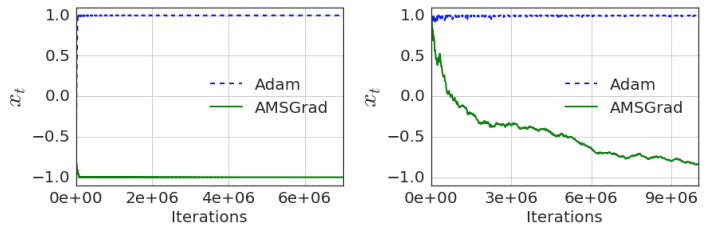
\includegraphics[width=1\linewidth]{OG_synthetic.png}
  \label{fig:test2}
\end{minipage}% 
\centering
\break
\begin{minipage}{0.9\textwidth}
  \centering
  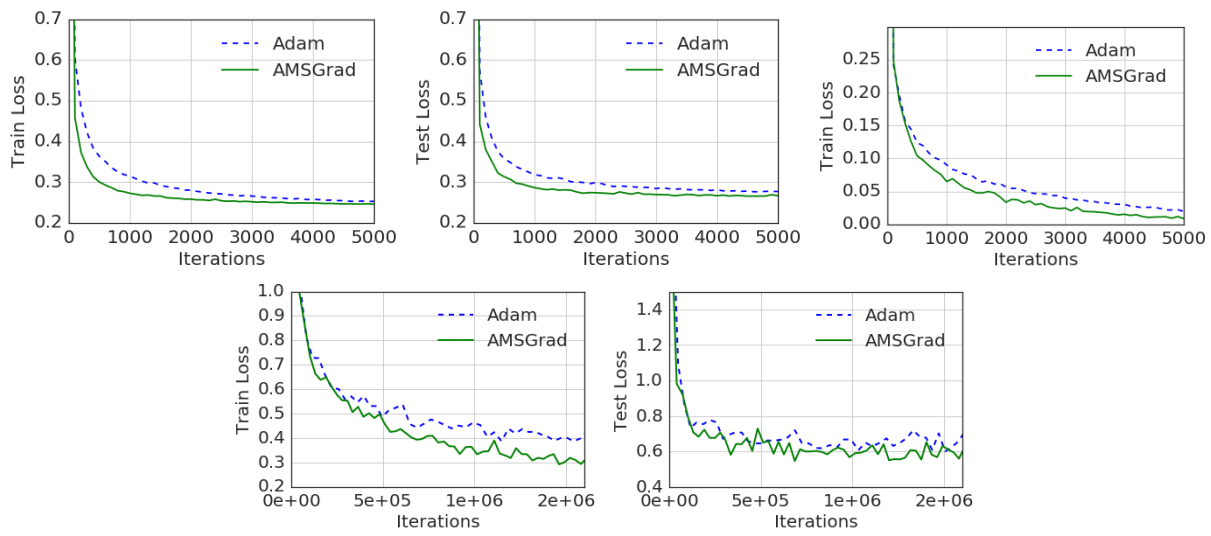
\includegraphics[width=1\linewidth]{OG_results_nets.png}
  \label{fig:test2}
\end{minipage}%
\end{minipage}
\caption[]{Top: location of $x_t$ in the online and stochastic syntetic experiments, respectively. \\
Middle: train and test loss of ADAM and AMSGrad on logistic regression (left and center) 1-hidden layer feedforward neural network (right) on MNIST.\\
Bottom: training and test loss of ADAM and AMSGrad with respect to iterations for CifarNet.\\
These graphs were taken directly from the paper \emph{On the Conergence of Adam and Beyond} (Sashank, Kale, Kumar; 2018).} 
\end{figure*}    

\section{METHODOLOGY}

In our experiments, we aimed to be faithful to the experimental setups the authors describe. Although the authors do not include all the details regarding their experiments (to be discussed, section VI), we emulated every design choice the authors reported. We implemented all our classifiers using \texttt{keras} (Chollet et. al; 2015) - which has implementations of the Adam and AMSGrad optimizers - and ran our grid searches using the \code{GridSearchCV} object and \code{KerasClassifier} wrapper from \texttt{sklearn} (Pedregosa et. al, 2011).


\subsection{Hyperparemter Tuning}

For each of the experiments regarding the MNIST and CIFAR-10 datasets, the authors describe the procedure they used to tune their model hyperparameters. For each model, they fix the batch size to $128$, and $\beta_1$ to $.99$. They state that they selected the learning rate $\alpha$ - without including a range of values they searched through - and $\beta_2$ from the range $(.99, .999)$, using an exhaustive grid search.

Thus, we also used a grid search to tune $\alpha$ and $\beta_2$ for the logistic regression, feedforward neural network, and CNN models. Although the authors do not specify the details of their grid search, we assumed that they were performing a variant of cross validation\footnote{We are comfortable with this assumption because is the standard procedure for hyperparameter tuning.} to select the best hyperparameters for each optimizer.

Since we were not initially aware of a neighborhood of values for $\alpha$ which work well for these models, nor how the learning rate $\alpha$ interacts with the smoothing parameter $\beta_2$, we experimented with five values for $\alpha$ of increasing orders of magnitude in our first grid searches. We also tried five different values of $\beta_2$ - yielding a parameter grid of 25 combinations:
\begin{gather*}
\alpha \in \{0.0001, 0.001, 0.01, 0.1, 1.0\} \\
\beta_2 \in \{0.99, 0.9925, 0.995, 0.9975, 0.999\}
\end{gather*}

We used this same parameter grid when tuning all of our models. 

Training the logistic regression and feedforward neural network models was relatively quick: on an NVIDIA Kepler GK104 GPU, one training epoch took around .5 seconds and 1 seconds, respectively. Thus, we simply ran an exhaustive grid search using 3-fold cross validation, totaling 75 fits for each model/optimizer combination. Each model was trained for 30 epochs for each fit. We selected the hyperparameters which yield the smallest validation loss. It took around 4 hours  to tune the hyperparameters for the logistic regression and feedforward nerual network models, using both AMSGrad and Adam. 

Tuning the learning hyperparameters $\alpha$ and $\beta_2$ was more expensive when using the CifarNet architecture (appendix 1). Each training epoch took around 90 seconds on this same hardware. It would take several days to tune the hyperparameters of this model with a similar exhaustive search.

Thus, we devised an abridged grid search procedure. First, we only trained the CifarNet models for 15 epochs when doing cross-validation. This short training period may introduce bias - favoring hyperparameters that yield quicker convergence (e.g. larger learning rates) - but it was necessary, given our computational constraints\footnote{We trained in the cloud using Amazon's AWS services. Lengthy processes become expensive, and we did not have funding for this project.}. We also enforced an early-stopping mechanism. During a training run, if the loss did not decrease for three consecutive epochs, then the run was terminated. This helped prevent unnecessarily training models using hyperparameters that are not fit for CifarNet. This modified grid search reduced the time to tune the hyperparameters $(\alpha, \beta_2)$ using CifarNet reduced to around 28 hours.

% Please add the following required packages to your document preamble:
% \usepackage[table,xcdraw]{xcolor}
% If you use beamer only pass "xcolor=table" option, i.e. \documentclass[xcolor=table]{beamer}
\begin{table}[]
\centering
\caption{Grid search results.}
\label{my-label}
\begin{tabular}{|
>{\columncolor[HTML]{DAE8FC}}c |
>{\columncolor[HTML]{ECF4FF}}c |c|c|}
\hline
\textbf{Experiment}                                                   & \cellcolor[HTML]{DAE8FC}\textbf{Optimizer} & \cellcolor[HTML]{DAE8FC}\textbf{$\alpha$} & \cellcolor[HTML]{DAE8FC}\textbf{$\beta_2$} \\ \hline
\begin{tabular}[c]{@{}c@{}}Logistic Regression\\ (MNIST)\end{tabular} & Adam                                       & 0.001                                     & 0.99                                       \\ \hline
\begin{tabular}[c]{@{}c@{}}Logistic Regression\\ (MNIST)\end{tabular} & AMSGrad                                    & 0.001                                     & 0.99                                       \\ \hline
\begin{tabular}[c]{@{}c@{}}Feedforward NN\\ (MNIST)\end{tabular}      & Adam                                       & 0.001                                     & 0.99                                       \\ \hline
\begin{tabular}[c]{@{}c@{}}Feedforward NN\\ (MNIST)\end{tabular}      & AMSGrad                                    & 0.001                                     & 0.999                                      \\ \hline
\begin{tabular}[c]{@{}c@{}}CifarNet \\ (CIFAR-10)\end{tabular}        & Adam                                       & 0.001                                     & 0.999                                      \\ \hline
\begin{tabular}[c]{@{}c@{}}CifarNet\\ (CIFAR-10)\end{tabular}         & AMSGrad                                    & 0.001                                     & 0.999                                      \\ \hline
\end{tabular}
\end{table}
\subsection{Reproduced Experiments}

Once we had tuned the values of $\alpha$ and $\beta_2$, we trained each of the models 5 times using the Adam optimizer and 5 times using the AMSGrad optimizer. For each training run, we recorded the training and test loss, as well as the training and test classification accuracy after every epoch [appendix 2].

\section{RESULTS}

\begin{figure*}
\begin{minipage}{1\textwidth}
  \centering
  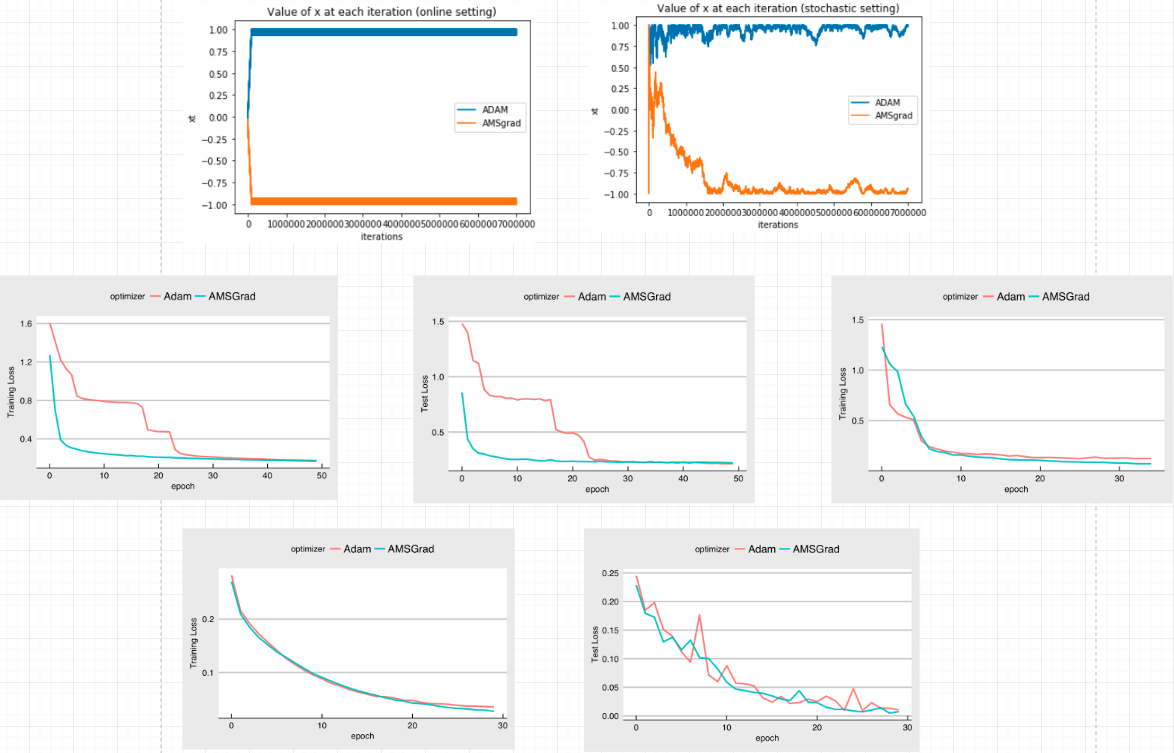
\includegraphics[width=1\linewidth]{Our_Results.png}
  \label{fig:test2}
\end{minipage}%
\caption[]{Results of recreated experiments. These training trajectories show the first of 5 created for each experiment, to mirror the authors' results presentation.\\
Top: location of $x_t$ in the online and stochastic synthetic experiments, respectively. \\
Middle: train and test loss of ADAM and AMSGrad on logistic regression (left and center) 1-hidden layer feedforward neural network (right) on MNIST.\\
Bottom: training and test loss of ADAM and AMSGrad with respect to iterations for CifarNet.\\.} 
\end{figure*}  

The results for our recreated experiments can be seen in Figure 2. In the synthetic experiments, our results for both the online and stochastic settings are virtually identical to the results presented in the paper. The only difference is that our AMSGrad converged more quickly to the optimal $x$ value than in the paper.

For the Logistic Regression experiment, we observe no discernible difference between the final training loss achieved by AMSGrad and the loss achieved by Adam. This result is similar to those reported by the paper. In contrast to the original results, however, we observe a more irregular training trajectory for the logistic regression model when trained with Adam. It appears the model reached a local optimum during training, before converging to a better optimum.

For the neural network experiments on MNIST and CIFAR-10, we found that AMSGrad yielded slightly lower training loss than Adam. Although the general trends of the training trajectories coincide with those found by the authors, we observed a smaller gap between the loss achieved by Adam and the loss achieved by AMSGrad. We also observed losses with magnitudes on a different scale than those reported by the authors, though this is likely because we do not use the same loss functions as the authors (to be discussed further in section VI).

\section{DISCUSSION AND CONCLUSION}

Although the authors take care to justify their claims with theory, there are several issues with their methodology and presentation of results, making it difficult to recreate their experiments exactly, and undermining their findings. These issues can be broadly categorized as:

\begin{enumerate}
\item Omitting key details in the experimental setup.
\item Failure to specify the model architectures completely.
\item Describing hyperparameter tuning procedures without specifying the values searched, or the final values found.
\item Failure to provide a sensitivity analysis of reported results.
\end{enumerate}

\subsection{Experimental Setup}

In the paper, the authors do not specify for how many epochs they trained each of the described classifiers.

Although the images they provide [Figure 1] show the number of \emph{iterations} they trained for, it is difficult to decipher what these iterations actually represent. 

For the models trained on MNIST, the authors show that they trained for 5,000 iterations. If an iteration is defined as one batch parameter update, then 5,000 iterations would correspond to 10-20 training epochs\footnote{The authors use mini-batches of size 128 in all experiments. Thus, in the $50,000$ training examples of MNIST, one epoch would consist of $50000/128 \approx 390$ batch parameter updates.}, which is reasonable. The authors show, however, that they trained CifarNet for over 2 million iterations. Using this same definition of an iteration, this would correspond to over $5,000$ training epochs. Given the size of CifarNet, we find it dubious that the authors trained for thousands of epochs\footnote{At 90 seconds per epoch, 1000 epochs would take over a day on an NVIDIA Kepler GK104 GPU.}.

To overcome this ambiguity, we determined a number of training epochs for each model that we found reasonable. We aimed to choose a number for each model that gives the model ample time to converge, but that can also train in a reasonable time frame. Thus, we trained our logistic regression and feedforward neural network models for 50 epochs and our CifarNet models for 30 epochs. 

\subsection{Model Architectures}

The authors do not specify several key details of their model architectures. Most severely, they do not specify the loss function they used to learn the model parameters. 

In a multi-class classification setting (such as MNIST and CIFAR-10 classification), a natural choice for a loss function is categorical cross-entropy. After running our experiments using categorical-crossentropy, however, we noticed that the scale of our models' losses did not match those reported by the authors. For example, when running a feedforward neural network on MNIST, we observed training losses in roughly the range (1, 6), while the authors report losses in the range (.2, .7). 

Based on these observations, we concluded that the authors must have used a loss function other than categorical-crossentropy. As an alternative, we tried using binary-crossentropy (also known as \emph{multiclass log-loss} in the multiclass setting), which is defined for a $k$ class classification problem as:

\[
Loss(\hat{y}_i, y_i) = -\sum_{k = 1}^K \big( y_{i,k}\log(\hat{y}_{i,k}) + (1 - y_{i,k})\log(1 - \hat{y}_{i,k})  \big)
\]

When using this loss function we found that our observed losses aligned more closely with those reported by the authors in our experiments regarding the MNIST dataset. However, we observed losses much smaller than those reported by the authors when training CifarNet. This could be because the authors used different loss functions in their experiments regarding MNIST and CIFAR-10. It could also be that the authors used a loss function other than categorical cross-entropy and multiclass log-loss.

As the paper's results focus on the superiority of AMSGrad over Adam, we decided that the magnitude of the losses observed is less important than the relative magnitude between those achieved when training with AMSGrad, and those achieved when training with Adam. Thus, we proceeded with our experiments using the multiclass log-loss, with knowledge that this loss may be different than the one used by the authors.

\subsection{Model Hyperparameters}

Finally, the authors do not go into full detail on the hyperparameters they chose for each model. 

In the CifarNet CNN model, an important hyperparameter is the stride length to use in each convolutional layer. Given just the kernel size and number of filters, one cannot deduce the stride length used by the authors\footnote{For the layer to be specified fully, either the stride length or zero-padding length should also be specified.}. Unable to resolve this ambiguity, we proceeded with our experiments using a stride length of one. Any discrepancies between our results and those reported by the author may be partly due to the use of different stride lengths. 

The authors mention that they tune the learning rate $\alpha$ and the hyperparameter $\beta_2$ using a grid search in each of their experiments. However, they do not specify the hyperparameters they ultimately used. 

This forced us to experiment with large parameter spaces when we recreated their grid searches, as we did not have an approximate neighborhood of values which we knew worked well in the proposed experiments. As training deep networks such as CifarNet is computationally intensive, exhaustive searches are costly. Thus, omitting the final hyperparameters introduces computational barriers to reproducing the authors' results. The grid search for CifarNet took about 28 hours to complete. This time could have been greatly reduced if the authors had given us the exact values of the best hyperparameters they found, or at least  a range for the $\alpha$ values they looked through. 

\subsection{Sensitivity Analysis of Results}

The authors present their results by displaying the loss trajectories during a single training run for each of the experiments described. Although their results seem conclusive, we do not think they are complete without addressing their sensitivity to changes in the underlying experimental conditions.

The authors' results are subject to random factors. The parameters in each of the models are randomly initialized\footnote{Although the authors do not explicitly specify how they initialized their model parameters, it is a widely acceptible practice to model parameters randomly and so we assume they did so.}, and in the CifarNet architecture, two dropout layers add even more stochasticity to the model. Thus, we can expect the learned parameters to vary between training runs, as well as the observed loss trajectories. Since the authors only report on one training run per model, we cannot gauge the variability amongst runs, nor how representative their results are of the expected training behavior. 

A natural way to address the randomness in the experiments is to train each model multiple times and report on the overall training patterns, as we have done (appendix 2). We observed that the training loss trajectories can vary quite significantly between runs as both Adam and AMSGrad are vulnerable to local optima. Further, in some runs of training the logistic regression classifier, we observed that Adam performed \emph{better} than AMSGrad - a result opposite to those reported by the authors. As the authors do not address the variability between runs, we cannot be sure if their results are definitive, or if they are a fluke.

In contrast to the authors' reported results, our experiments suggest that AMSGrad has only a modest advantage over Adam. The only experiment in which we found that AMSGrad indubitably performs better than Adam is the synthetic experiment. This is not surprising, as this experiment constructs a setting designed so that Adam would fail. The authors do not speak to how commonplace or exceptional such settings are, and so one cannot know how readily these results will extend to new datasets. It would have made their results more robust if they had discussed settings in which they believe their results do not apply.

\section{STATMENT OF CONTRIBUTION}

Emmanuel reproduced the experiments regarding the synthetic datasets, and anlyzed the results. Tamir reproduced the experiments regarding the MNIST and CIFAR-10 datasets, and contributed to this paper. L\'ea  focused on writing this paper. 
 
\addtolength{\textheight}{-12cm}   % This command serves to balance the column lengths
                                  % on the last page of the document manually. It shortens
                                  % the textheight of the last page by a suitable amount.
                                  % This command does not take effect until the next page
                                  % so it should come on the page before the last. Make
                                  % sure that you do not shorten the textheight too much.

%%%%%%%%%%%%%%%%%%%%%%%%%%%%%%%%%%%%%%%%%%%%%%%%%%%%%%%%%%%%%%%%%%%%%%%%%%%%%%%%



%%%%%%%%%%%%%%%%%%%%%%%%%%%%%%%%%%%%%%%%%%%%%%%%%%%%%%%%%%%%%%%%%%%%%%%%%%%%%%%%
\begin{thebibliography}{99}
\bibitem{c1} R. Sashank, S. Kale, S. Kumar, (2018). On the Convergence of Adam and Beyond. In Proceedings of \emph{International Conference on Learning Representations}, http://https://openreview.net/forum?id=ryQu7f-RZ (link is external)
\bibitem{c2} Diederik P. Kingma and Jimmy Ba (2015). Adam: A method for stochastic optimization. In Proceedings
of \emph{3rd International Conference on Learning Representations, 2015.}
\bibitem{c3} Chollet, Fran\c{c}ois and others, 2015. Keras: \url{https://keras.io}
\bibitem{c4} T. Tieleman and G. Hinton. RmsProp: Divide the gradient by a running average of its recent magnitude.
\bibitem{c5} John C. Duchi, Elad Hazan, and Yoram Singer. Adaptive subgradient methods for online learning
and stochastic optimization. Journal of Machine Learning Research, 12:2121–2159, 2011.
\bibitem{c6} Pedregosa, F. et al. Scikit-learn: Machine Learning in Python. \emph{Journal of Machine Learning Research}, 2011;


\section*{Blog Posts}

\bibitem{c7} Brownlee, J. (2016, August 9). Tuning optimization parameters using a gridsearch. Retrieved from https://machinelearningmastery.com/grid-search-hyperparameters-deep-learning-models-python-keras/
\bibitem{c8} Korzeniowski, F. (2017, December 22). Experiments with AMSGrad. Retrieved from https://fdlm.github.io/post/amsgrad/

\end{thebibliography}
\newpage
\section{APPENDIX}
\large{Appendix 1: Model Architectures}

\begin{figure}[H]
      \centering
      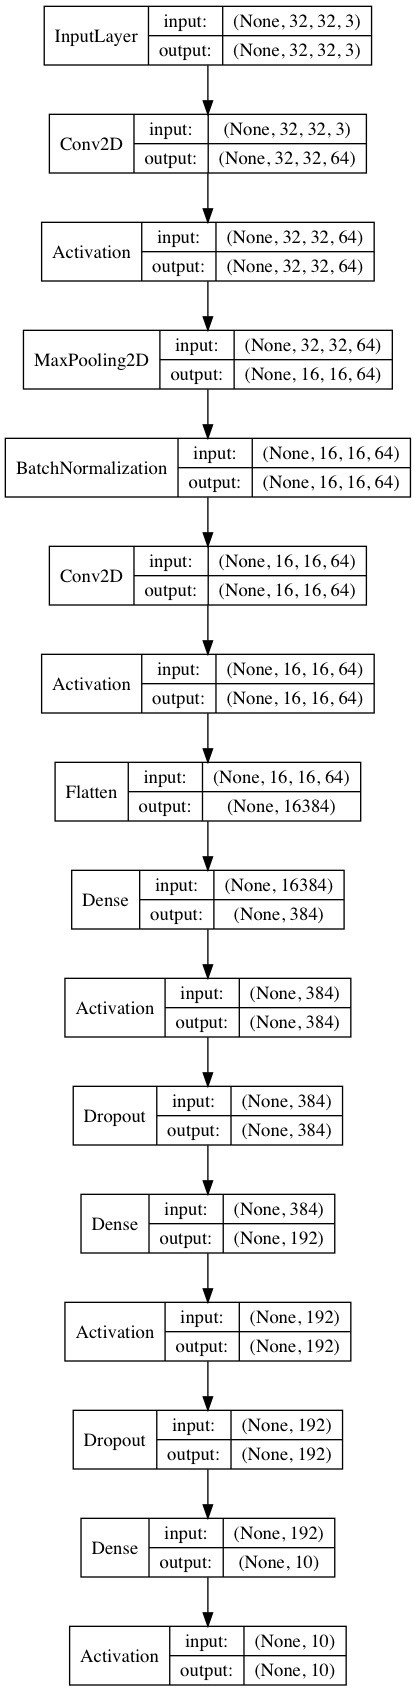
\includegraphics[scale = .3]{cifarnet_model.png}
		\centering
      %\includegraphics[scale=1.0]{figurefile}
      \caption{CifarNet architecture; a deep Convolutional Neural Network designed to classify images in the Cifar-10 dataset.}
      \label{figurelabel}
\end{figure}
    
\begin{figure}[H]
      \centering
      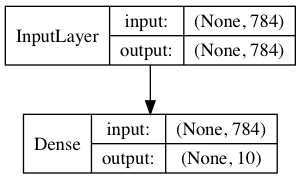
\includegraphics[scale = .3]{logreg_model.png}
		\centering
      \caption{Logistic Regression model, implemented as a feedforward neural network with no hidden layers.}
      \label{figurelabel}
\end{figure}

\begin{figure}[H]
      \centering
      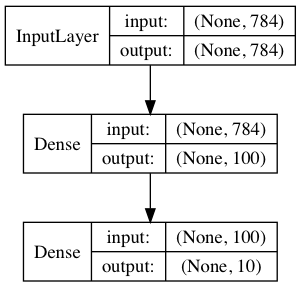
\includegraphics[scale = .3]{ffnn_model.png}
		\centering
      %\includegraphics[scale=1.0]{figurefile}
      \caption{Feedforward Neural Network Architecture, trained on MNIST 28x28 greyscale images.}
      \label{figurelabel}
\end{figure}

\hrulefill

\large{Appendix 2: Repeated Training Runs}

\begin{figure*}
\centering
\begin{tabular}{cccc}
\subfloat{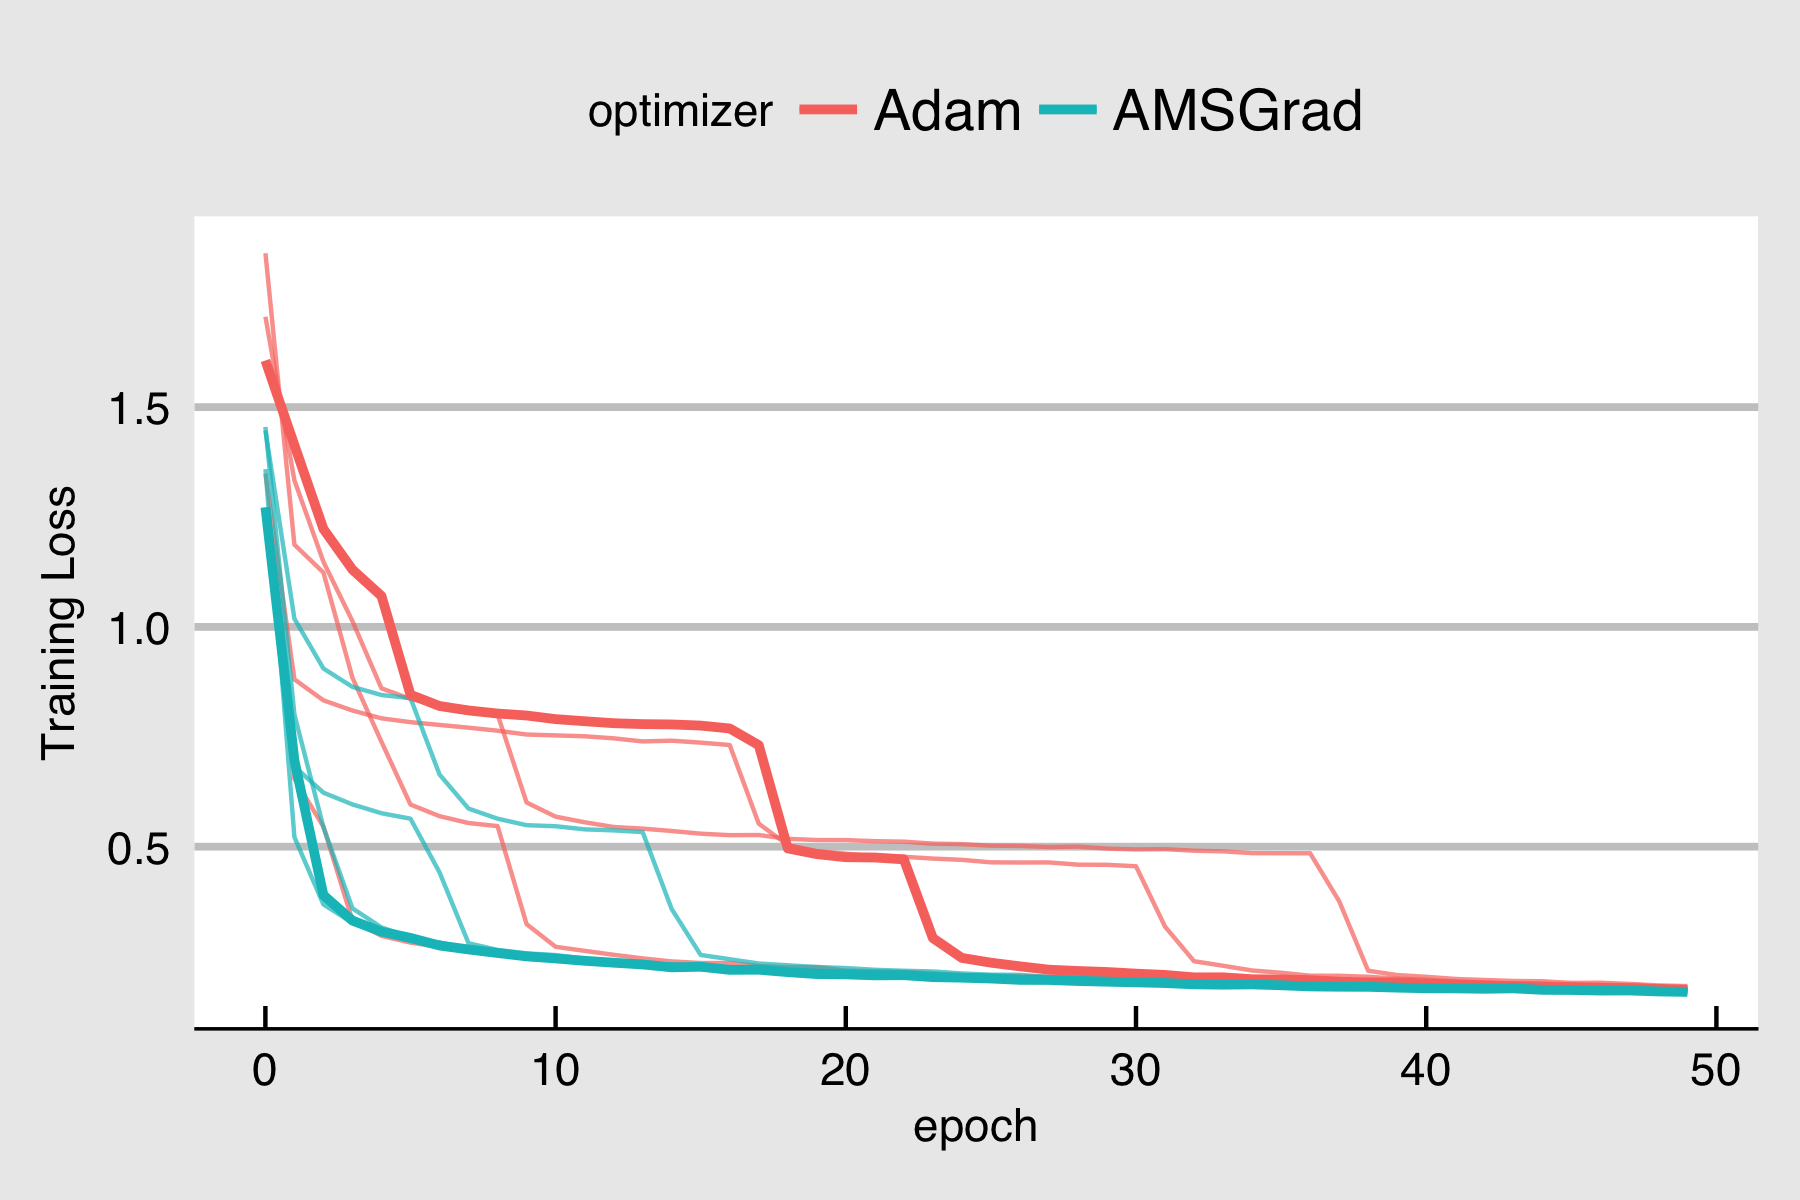
\includegraphics[width = 3in]{logreg_multi_trainloss}} &
\subfloat{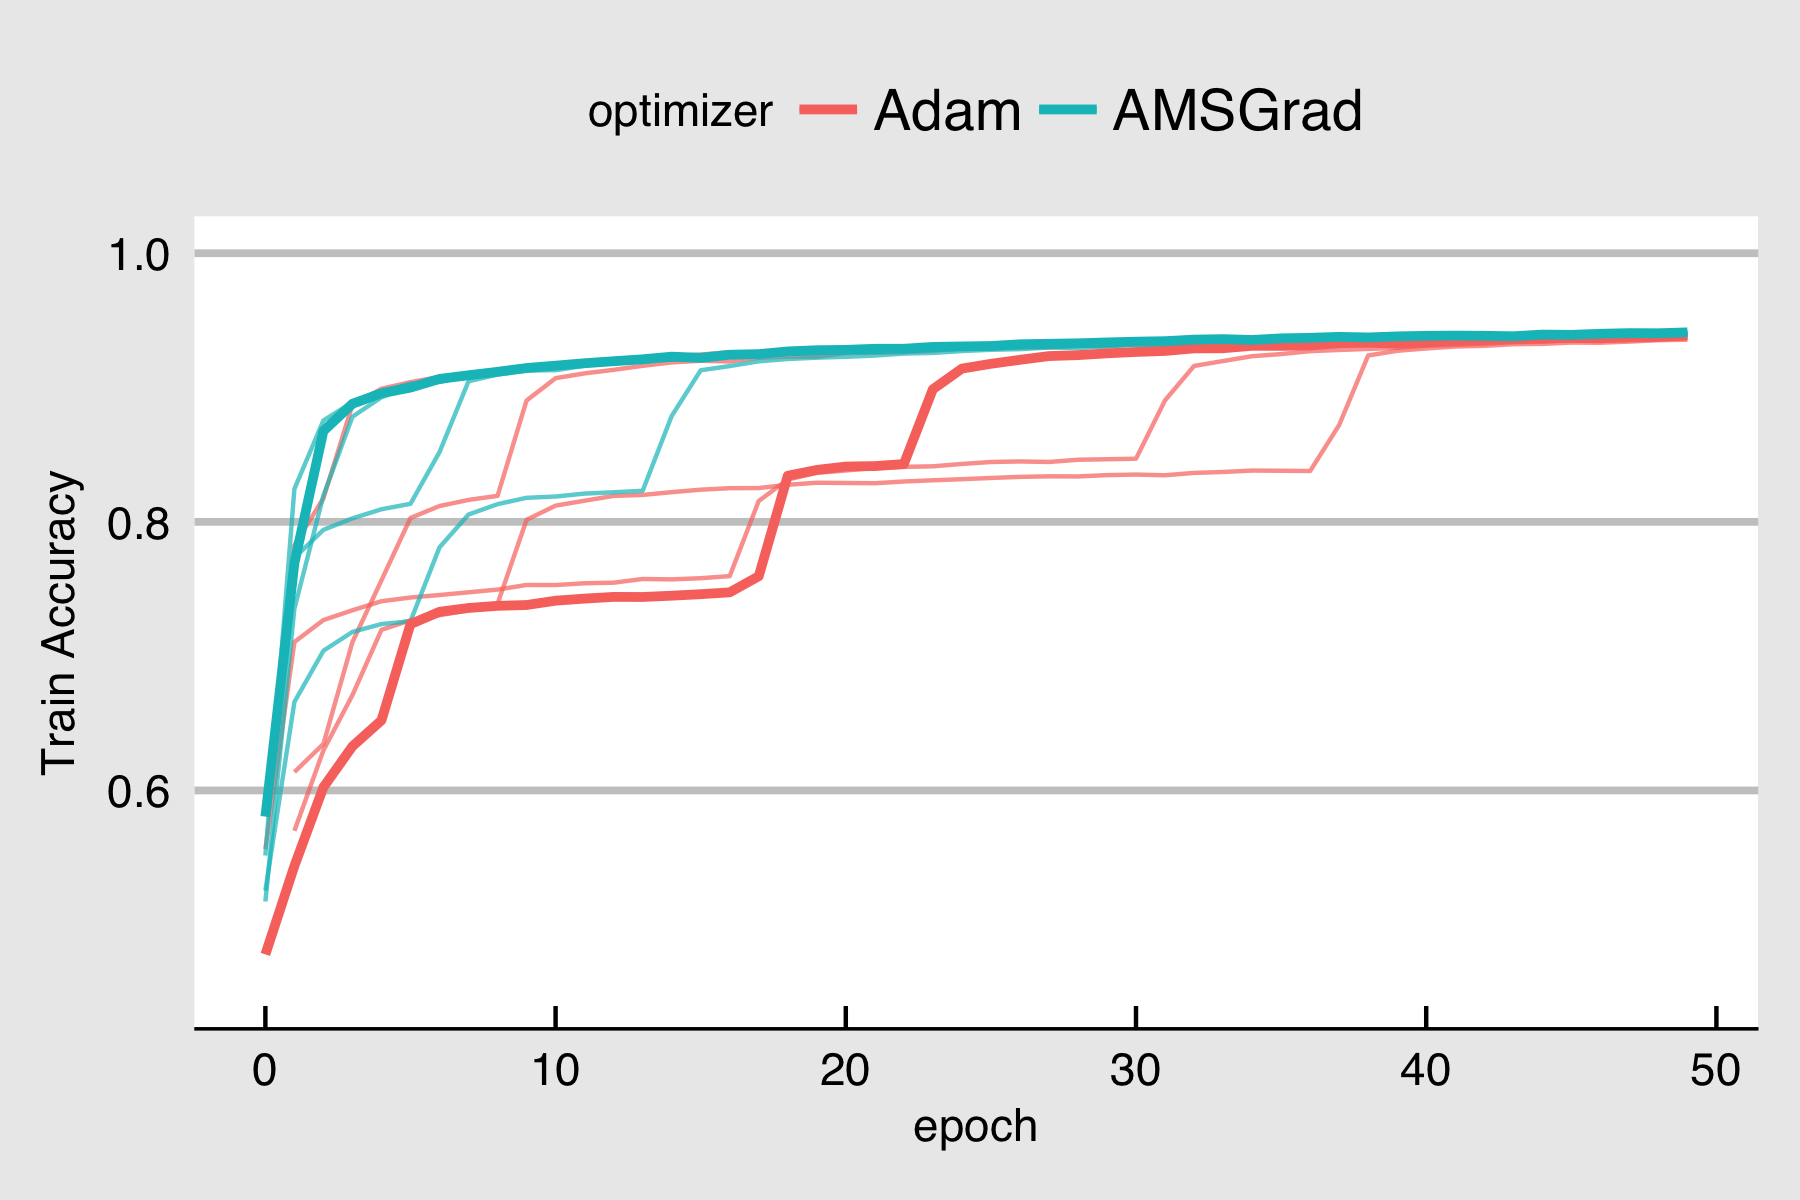
\includegraphics[width = 3in]{logreg_multi_train_acc}} \\
\subfloat{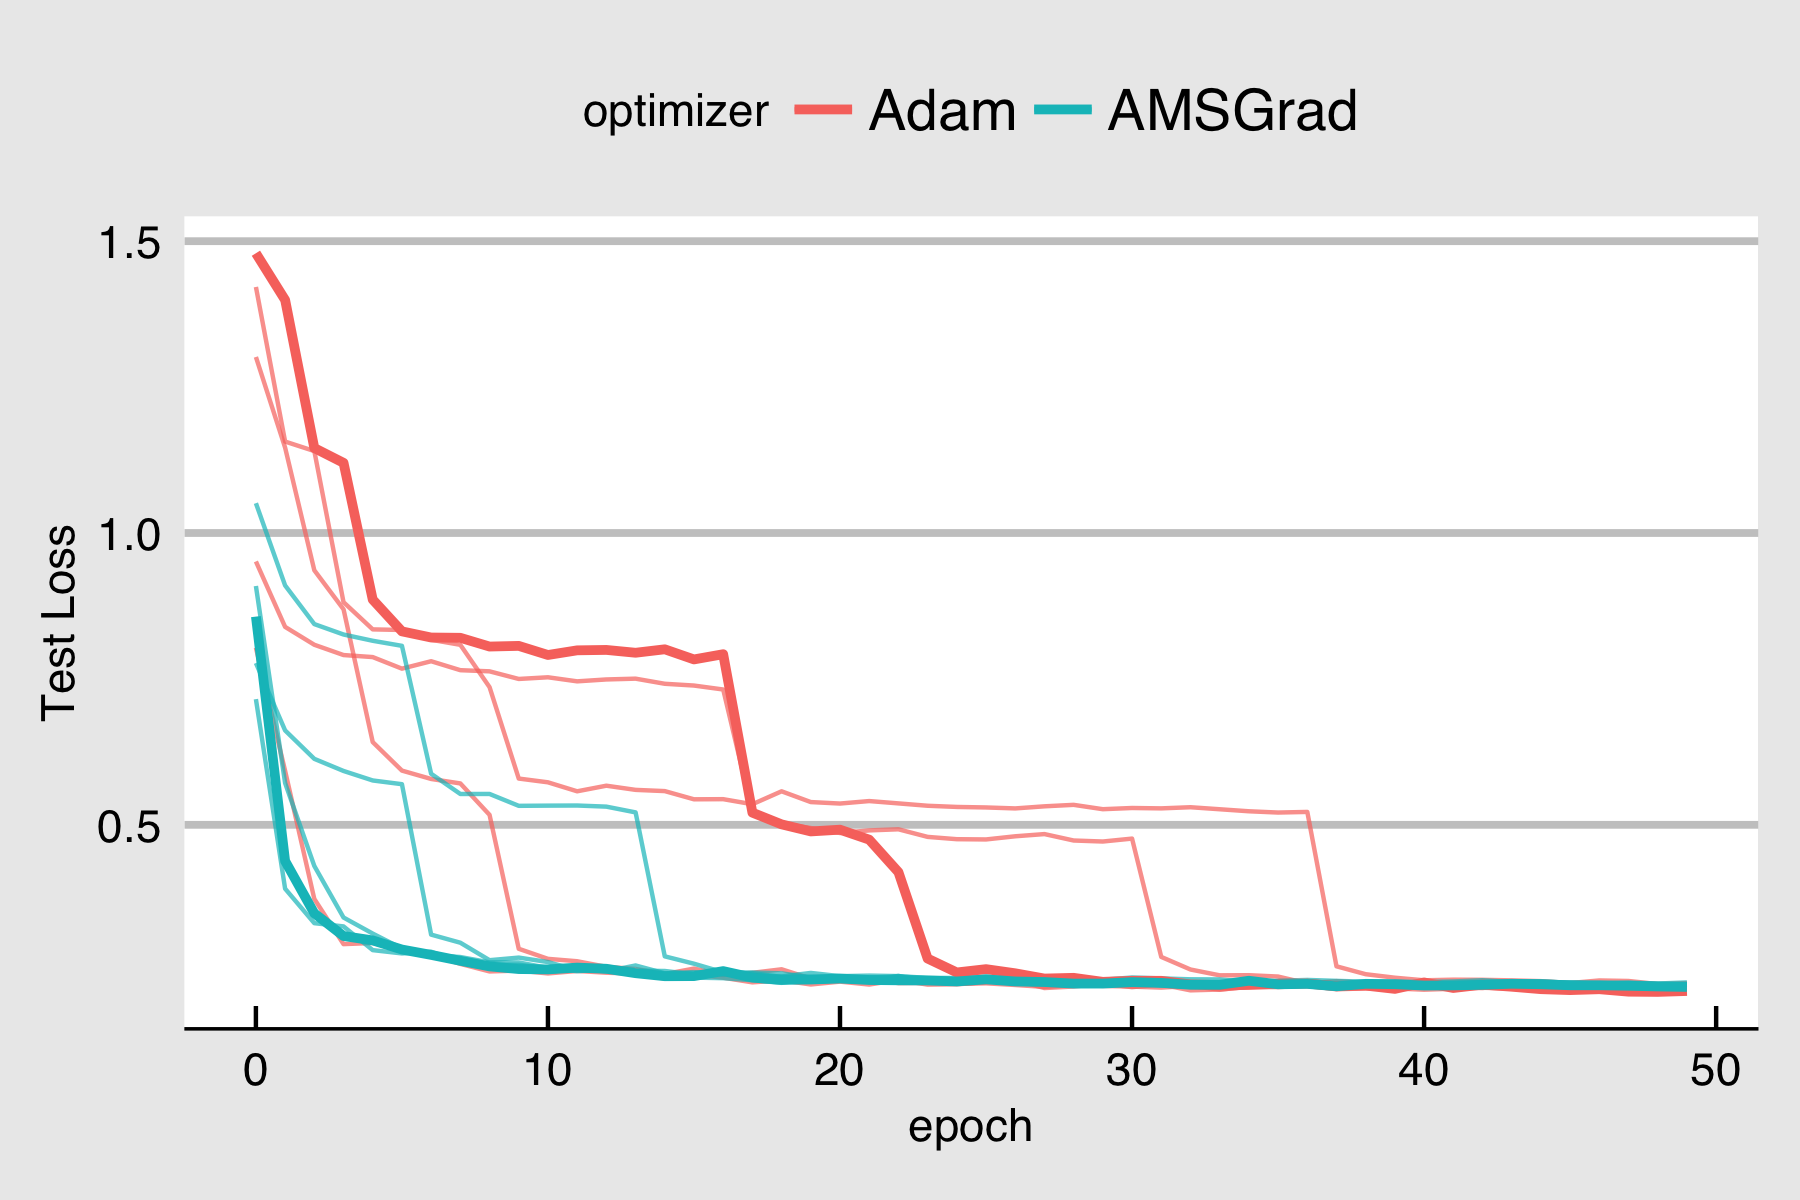
\includegraphics[width = 3in]{logreg_multi_testloss}} &
\subfloat{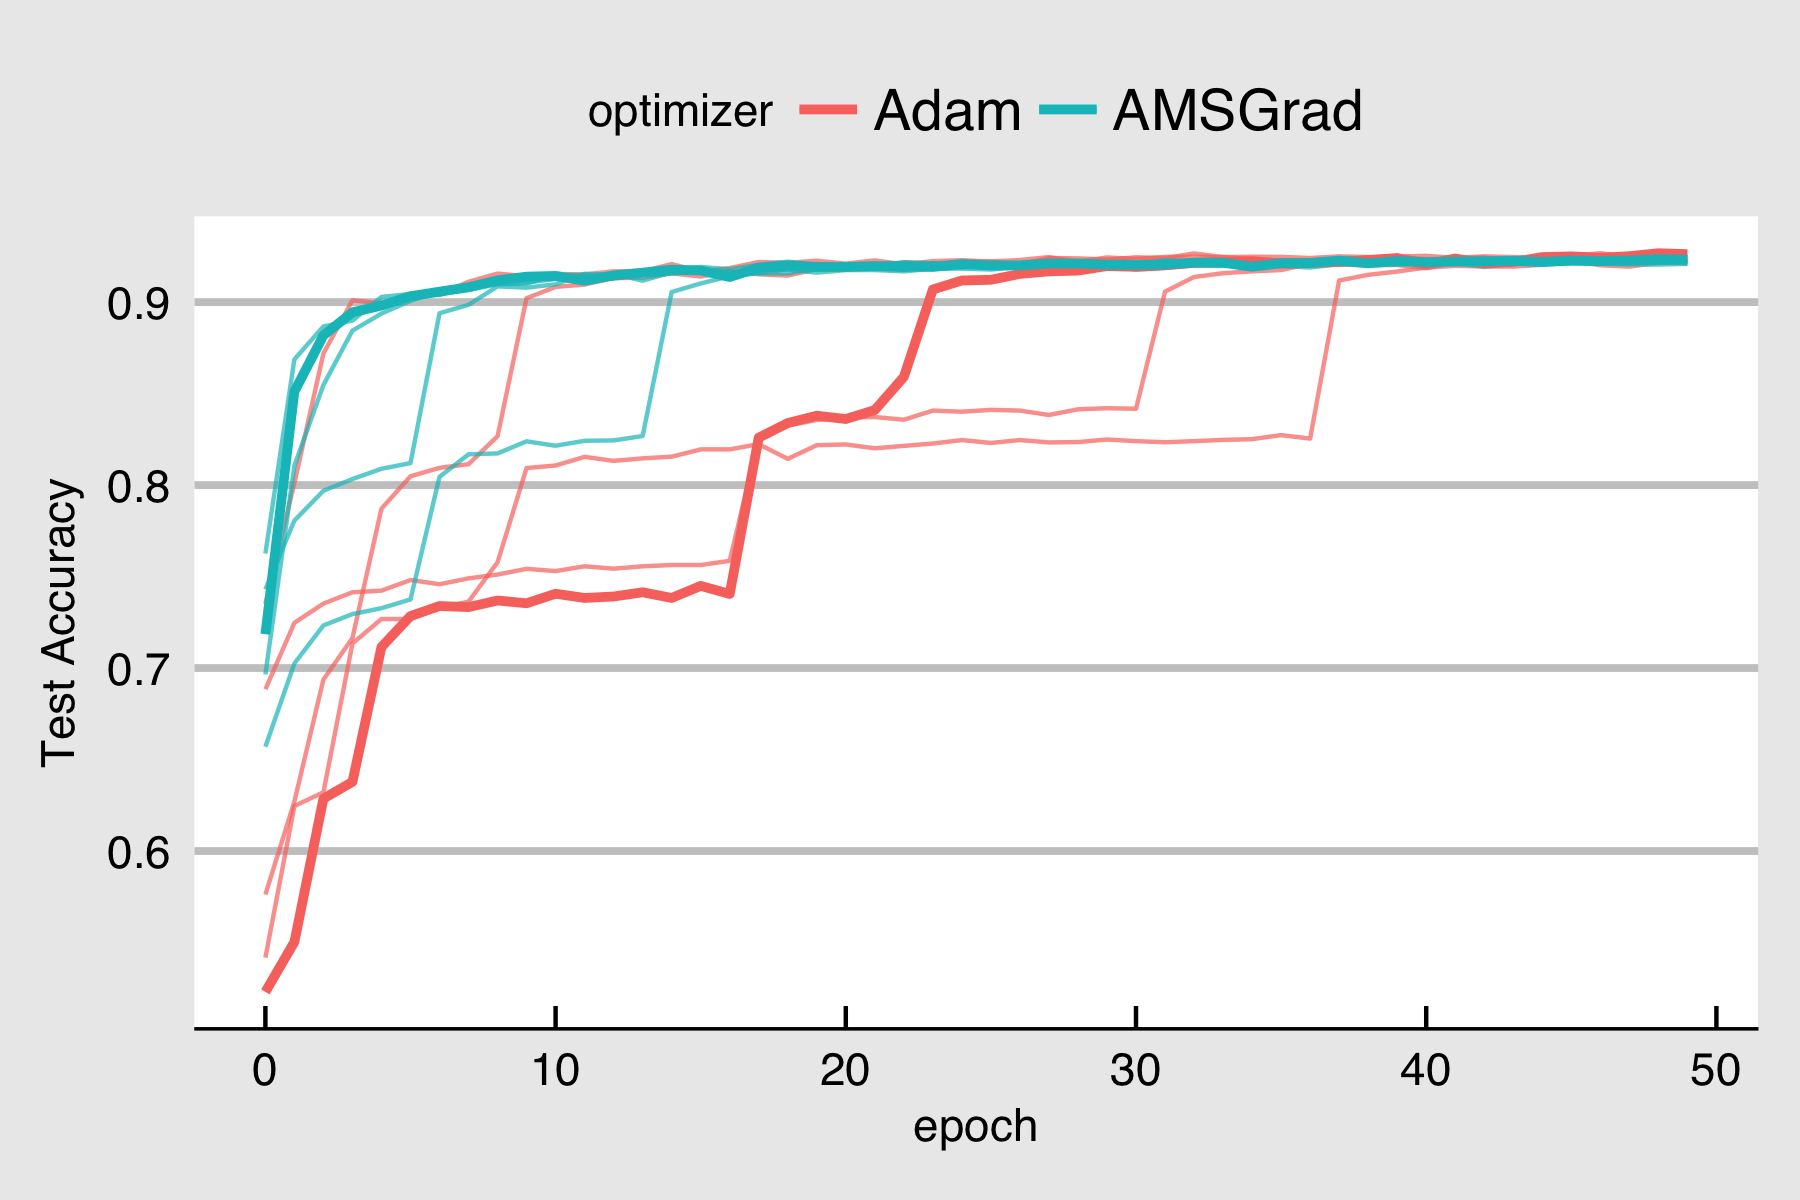
\includegraphics[width = 3in]{logreg_multi_test_acc}}
\end{tabular}
\caption{Training trajectories of Logistic Regression model on MNIST. The first run observed is in bold.\\
Top: training loss and accuracy. Bottom: test loss and accuracy.}
\end{figure*}

\begin{figure*}
\centering
\begin{tabular}{cccc}
\subfloat{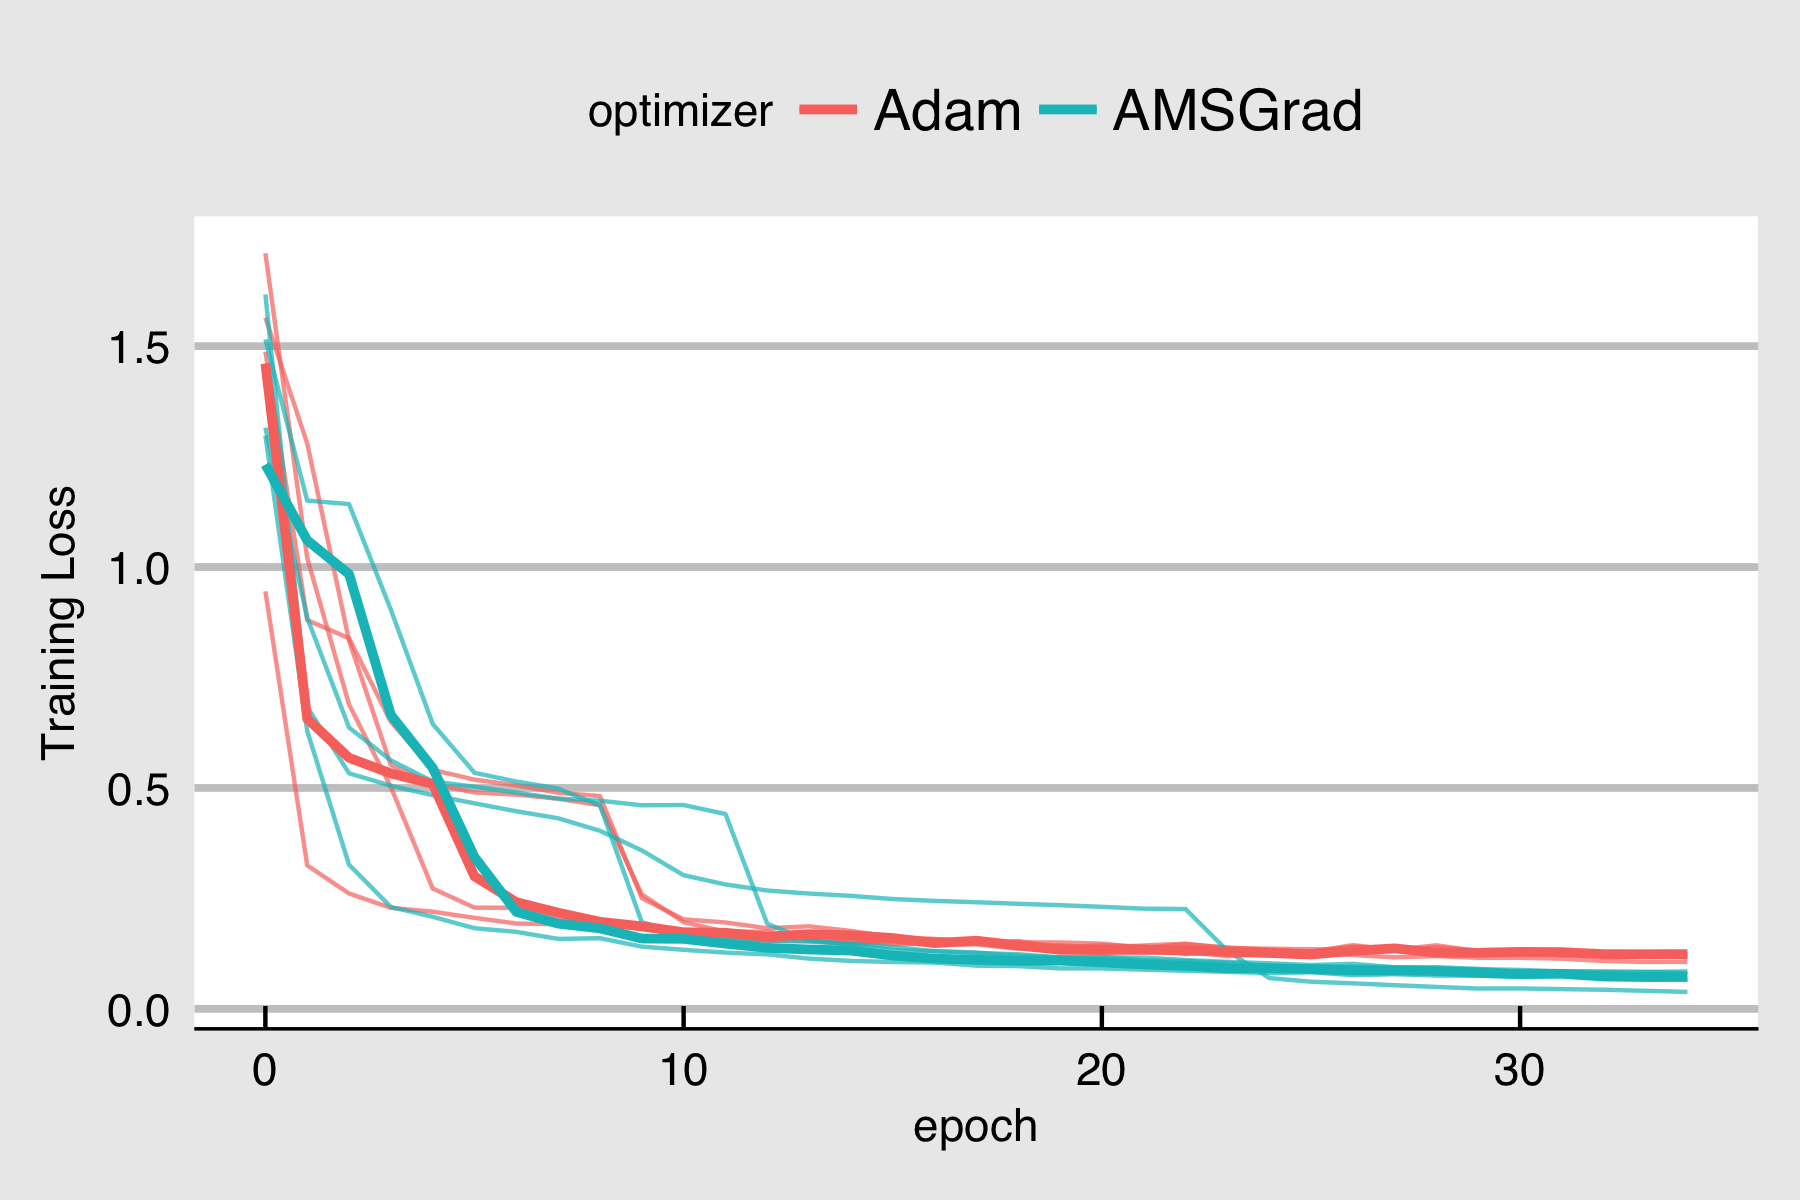
\includegraphics[width = 3.1in]{ffnn_multi_trainloss}} &
\subfloat{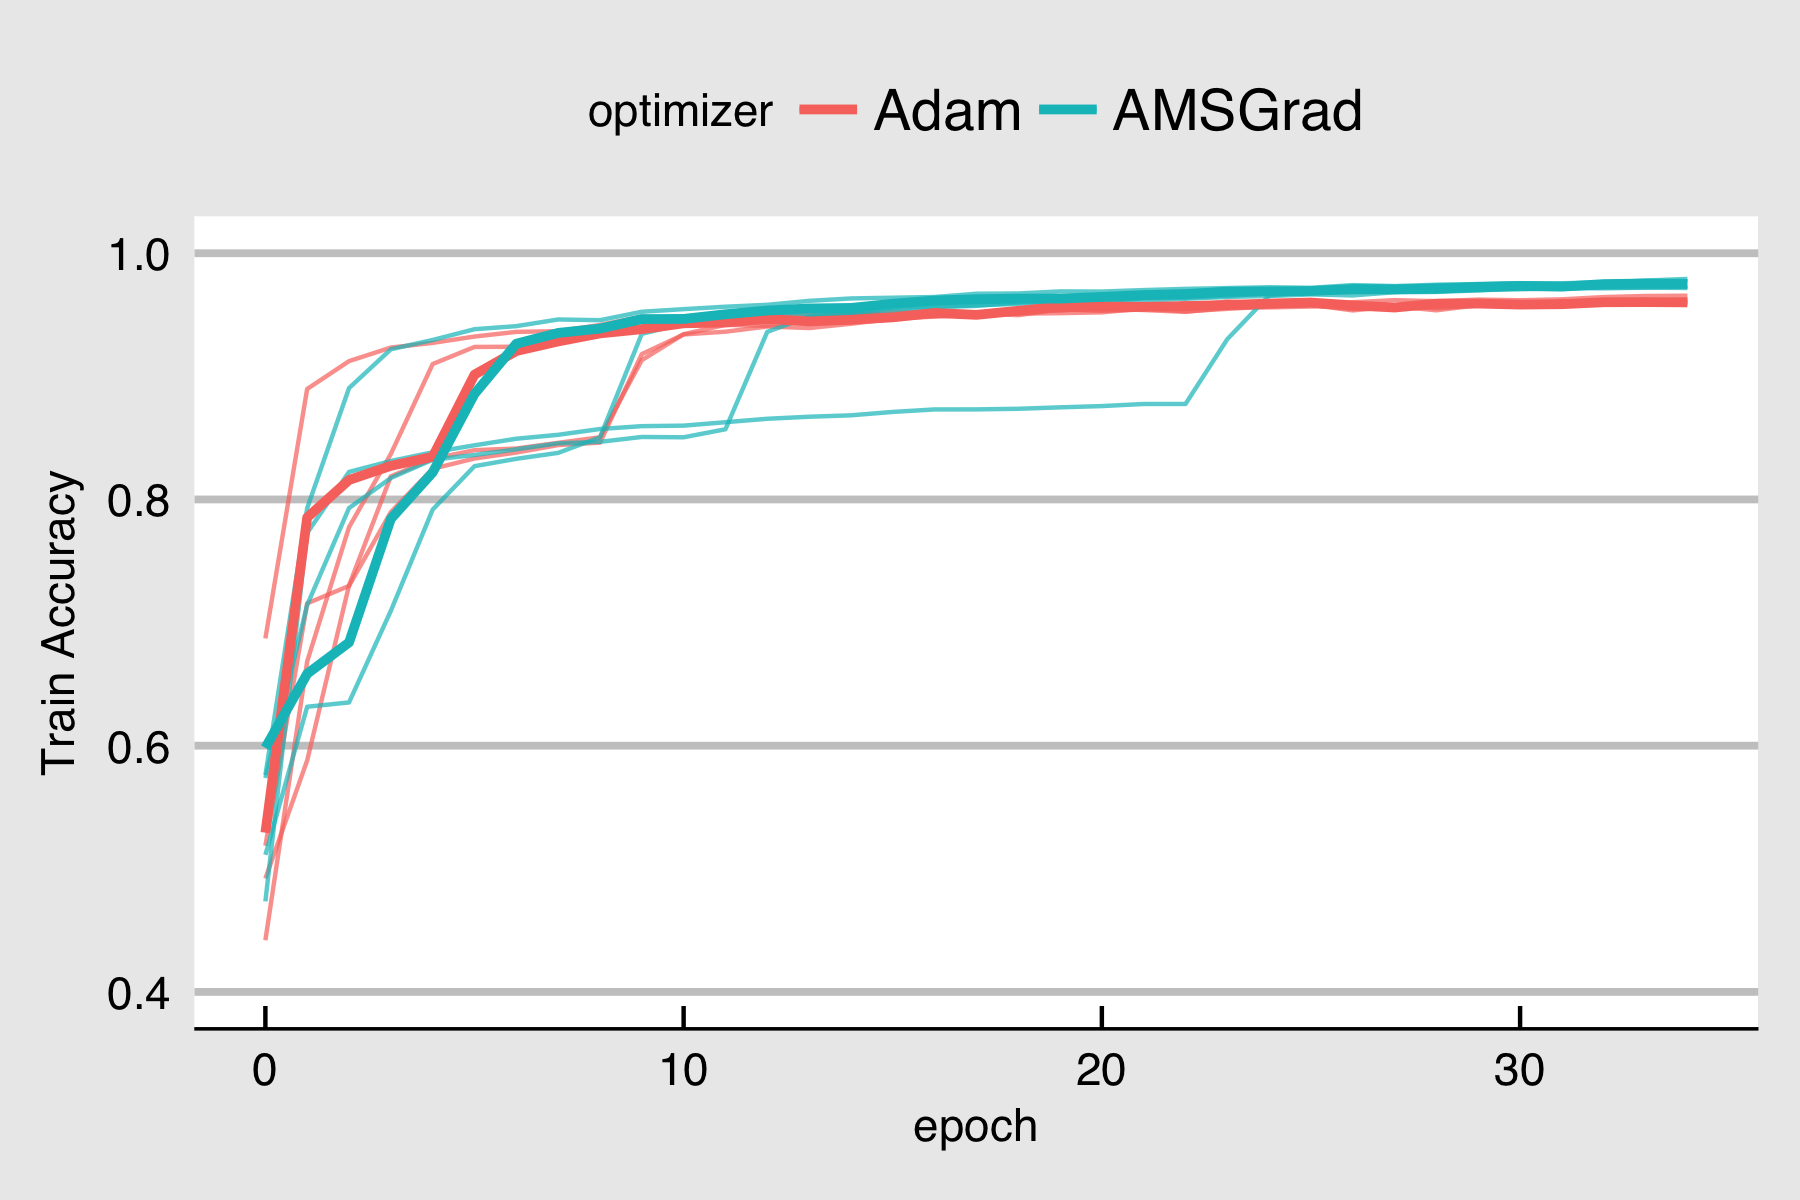
\includegraphics[width = 3.1in]{ffnn_multi_train_acc}} \\
\subfloat{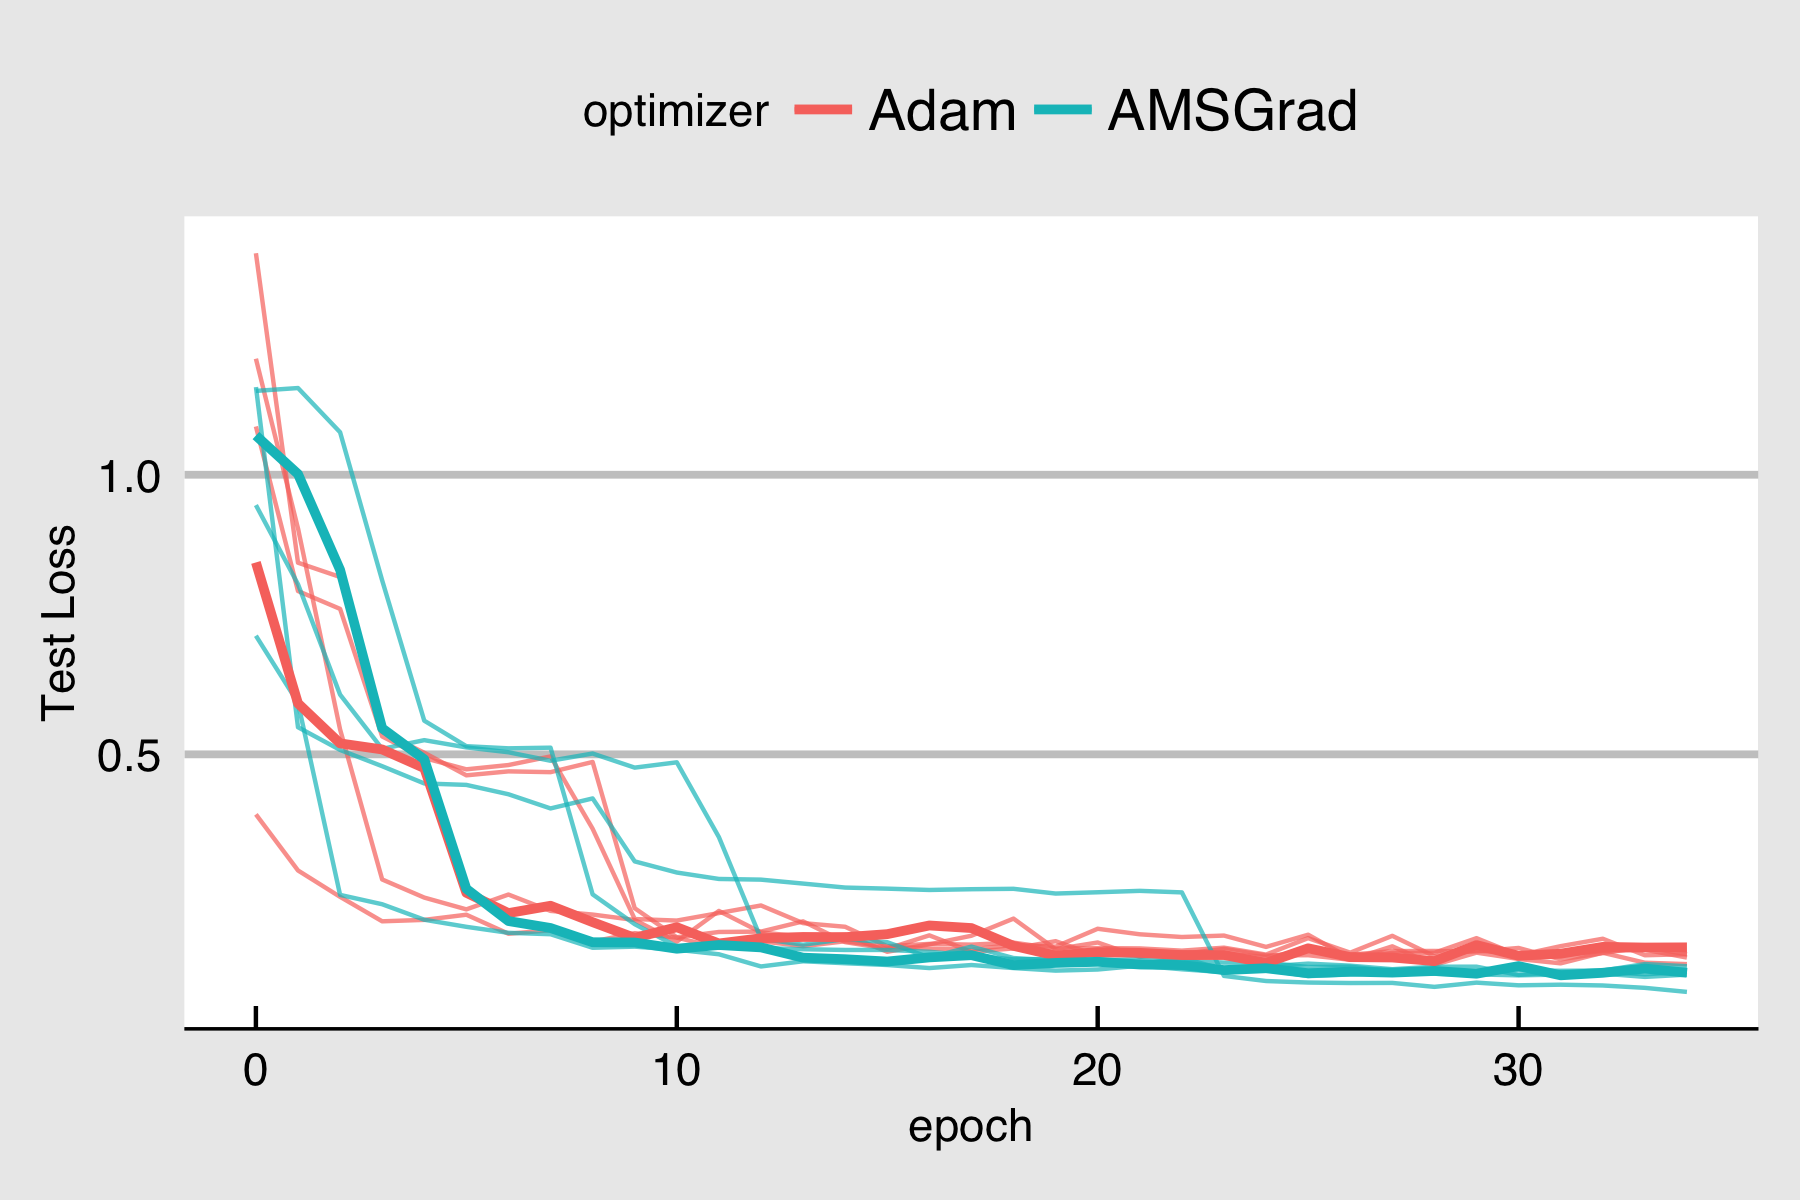
\includegraphics[width = 3.1in]{ffnn_multi_testloss}} &
\subfloat{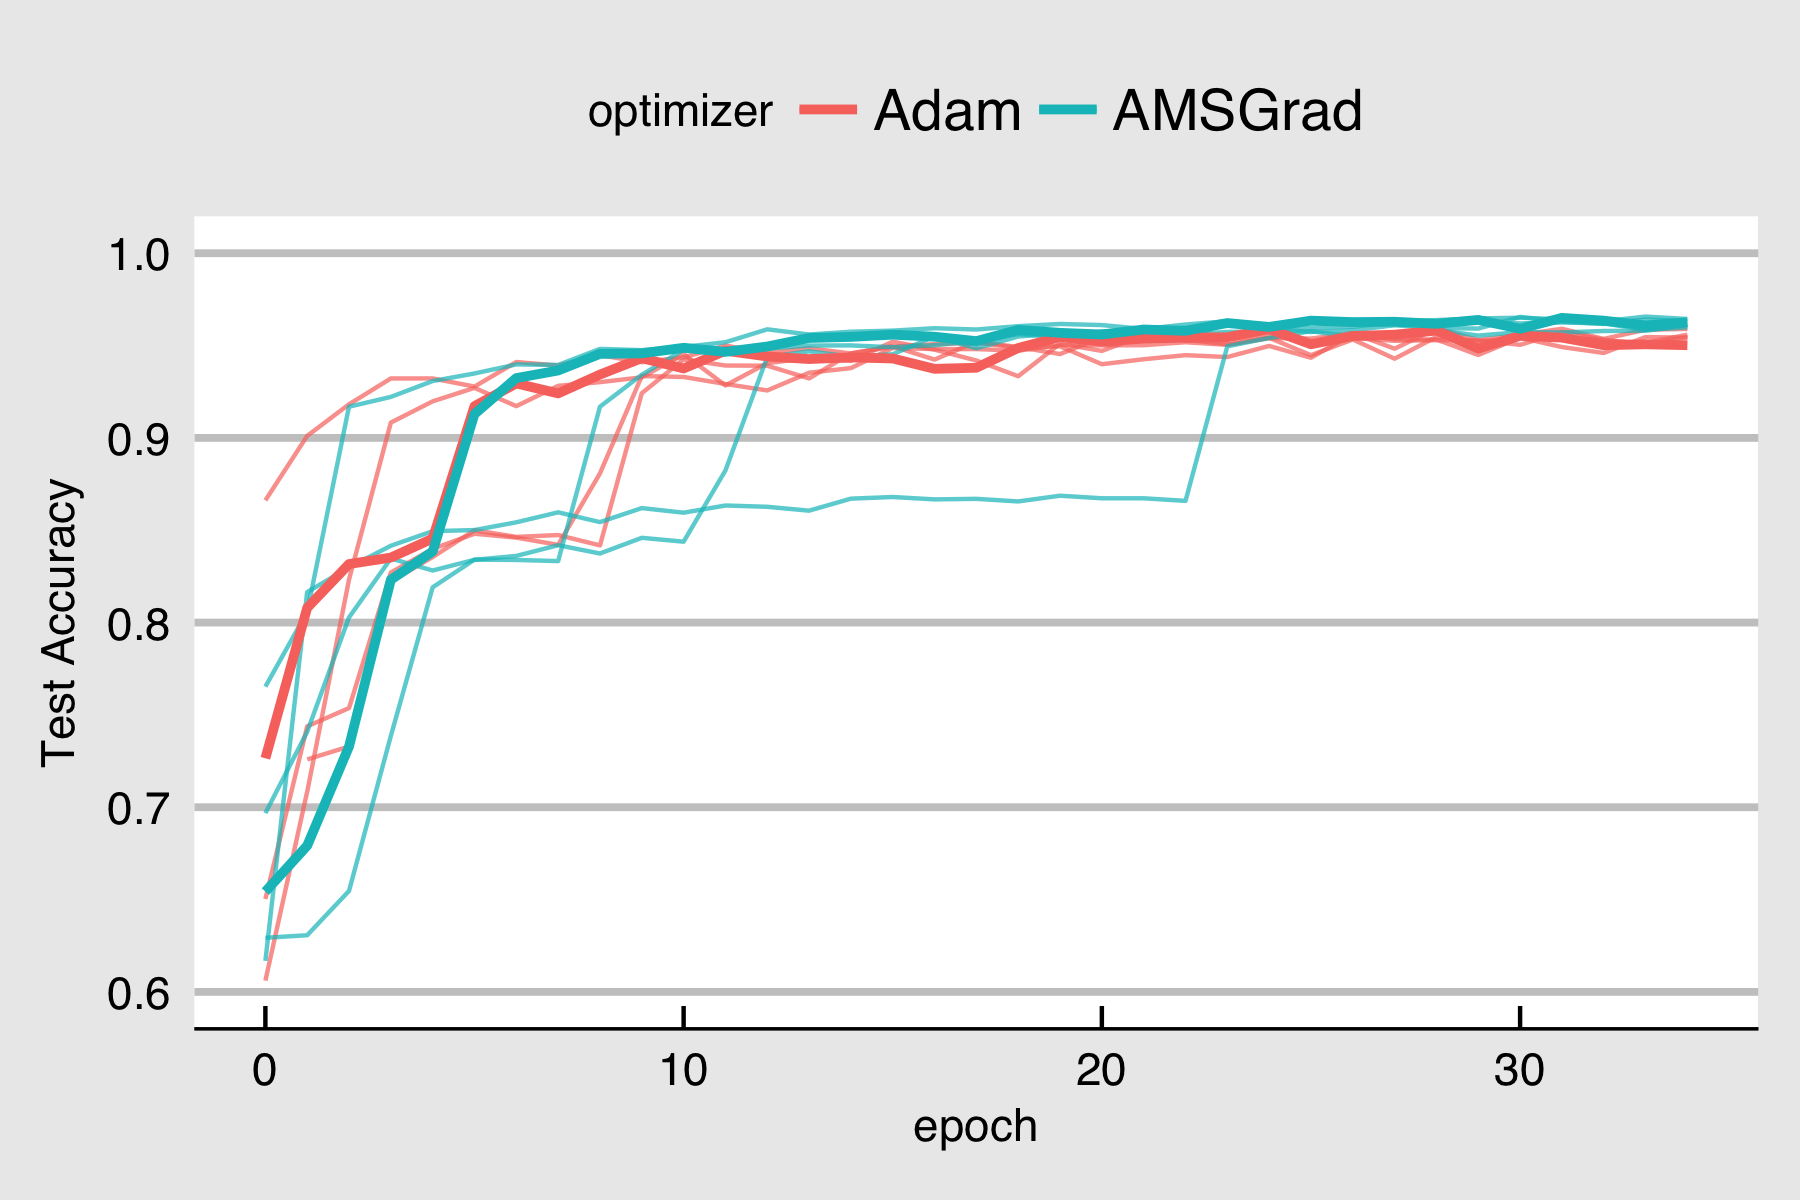
\includegraphics[width = 3.1in]{ffnn_multi_test_acc}}
\end{tabular}
\caption{Training trajectories of Feedforward Neural Network model on MNIST. The first run observed is in bold.\\
Top: training loss and accuracy. Bottom: test loss and accuracy.}
\end{figure*}

\begin{figure*}
\centering
\begin{tabular}{cccc}
\subfloat{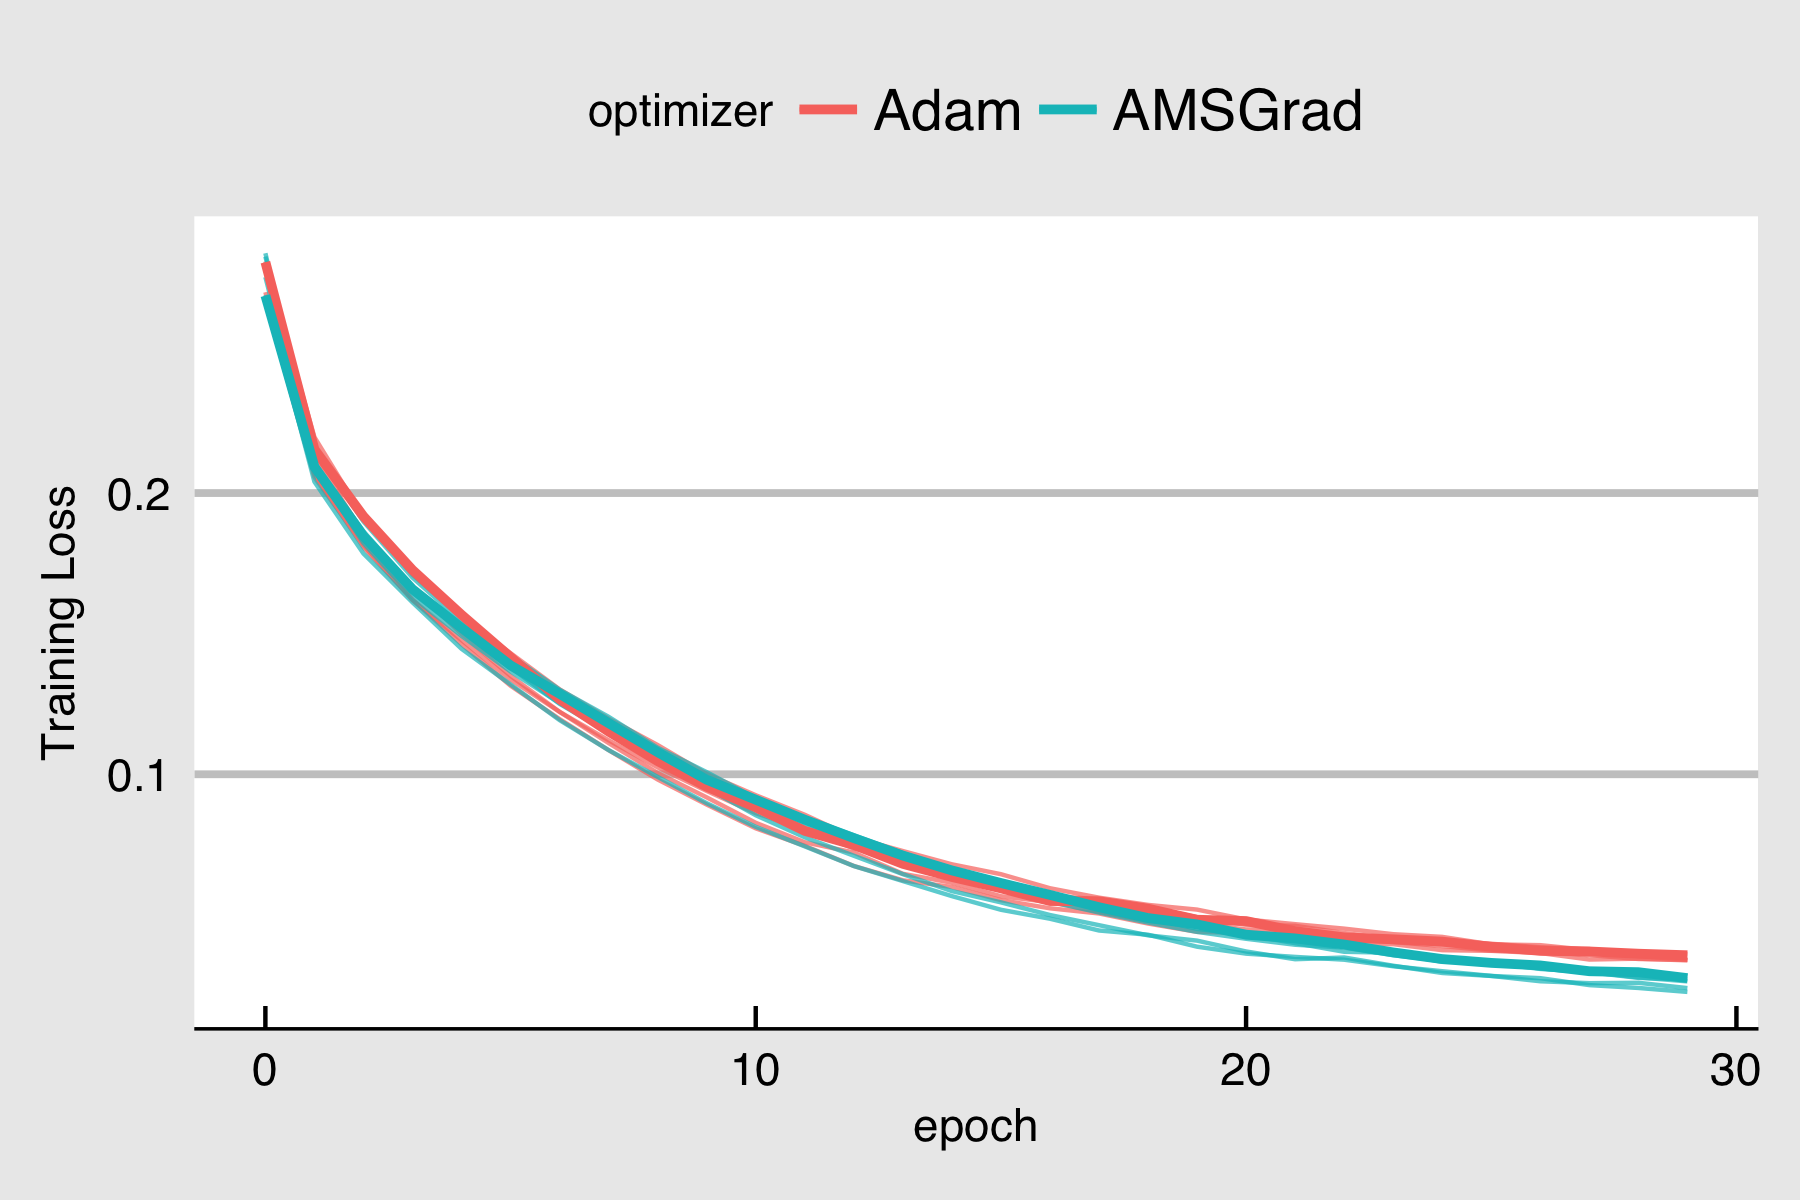
\includegraphics[width = 3.1in]{cifar_multi_trainloss}} &
\subfloat{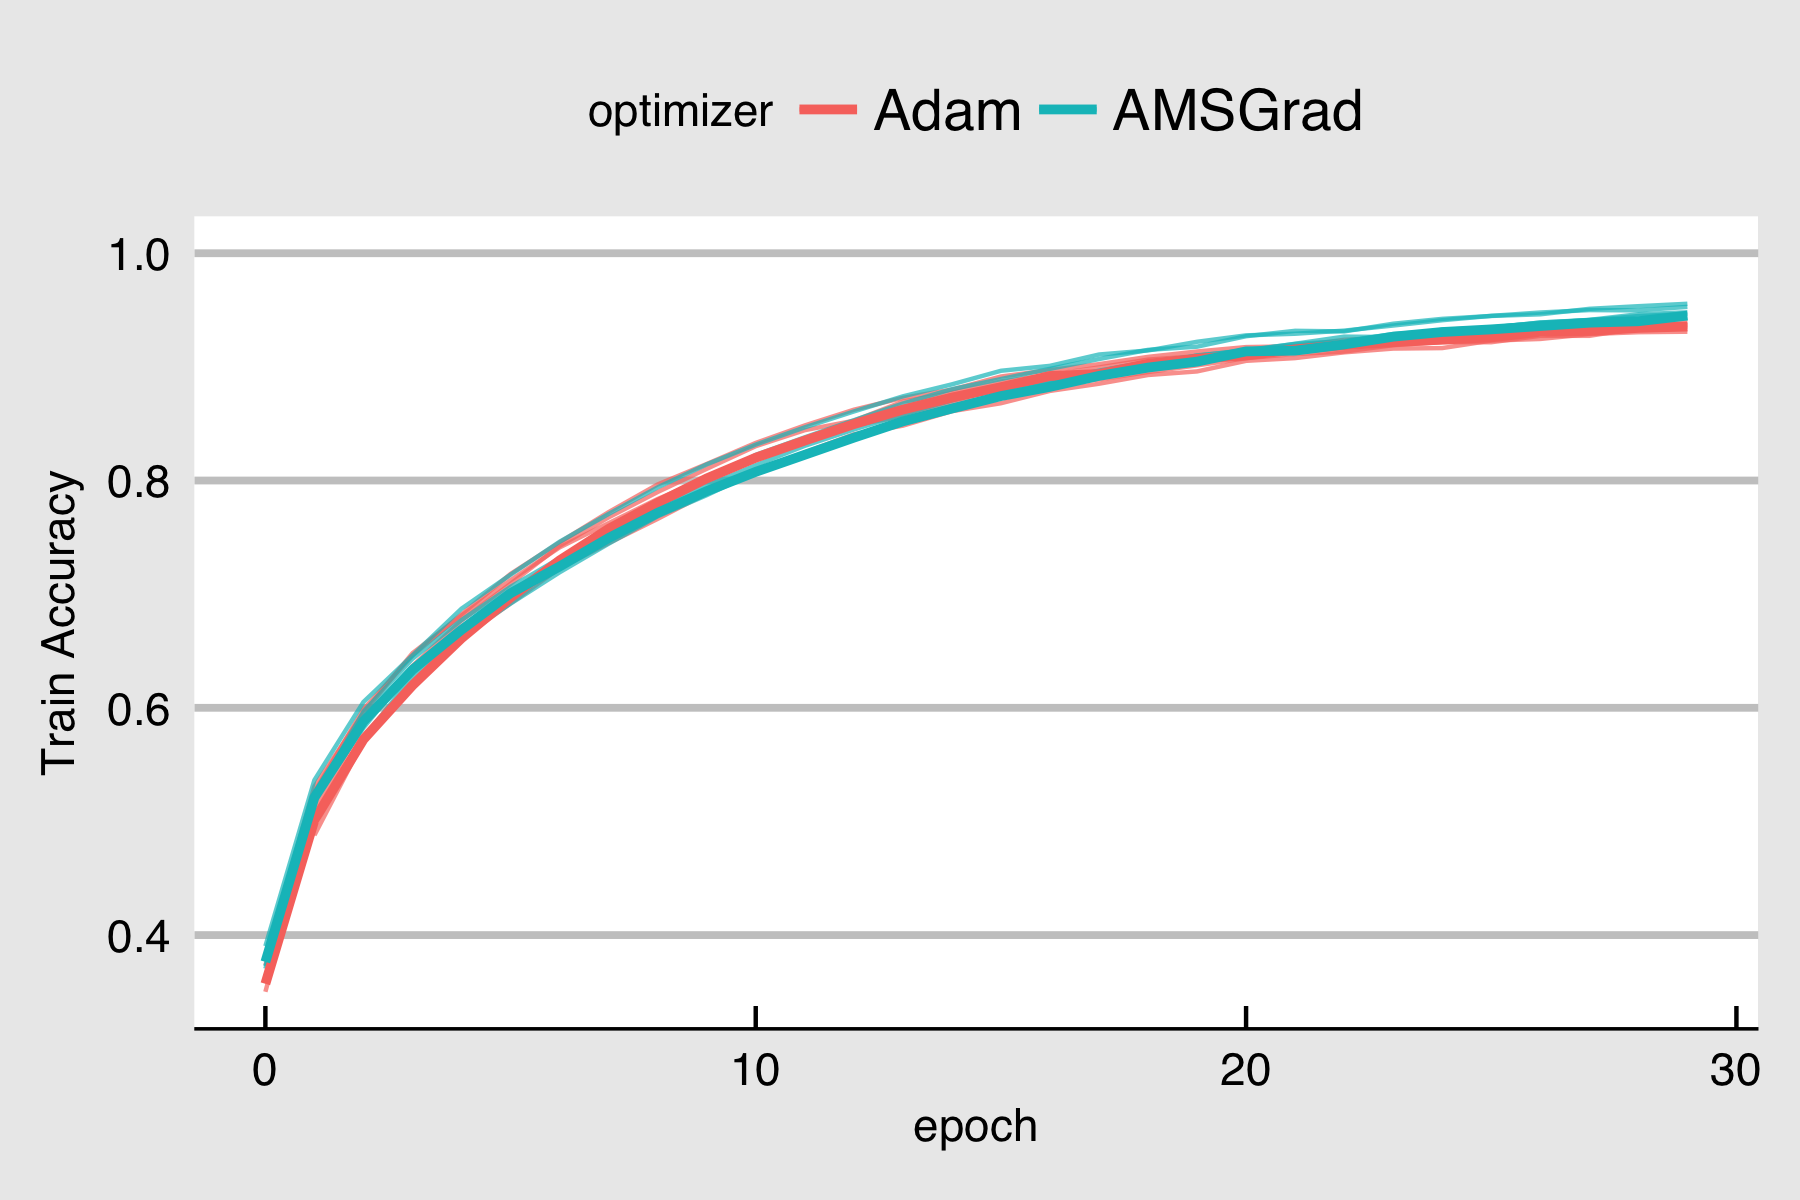
\includegraphics[width = 3.1in]{cifar_multi_train_acc}} \\
\subfloat{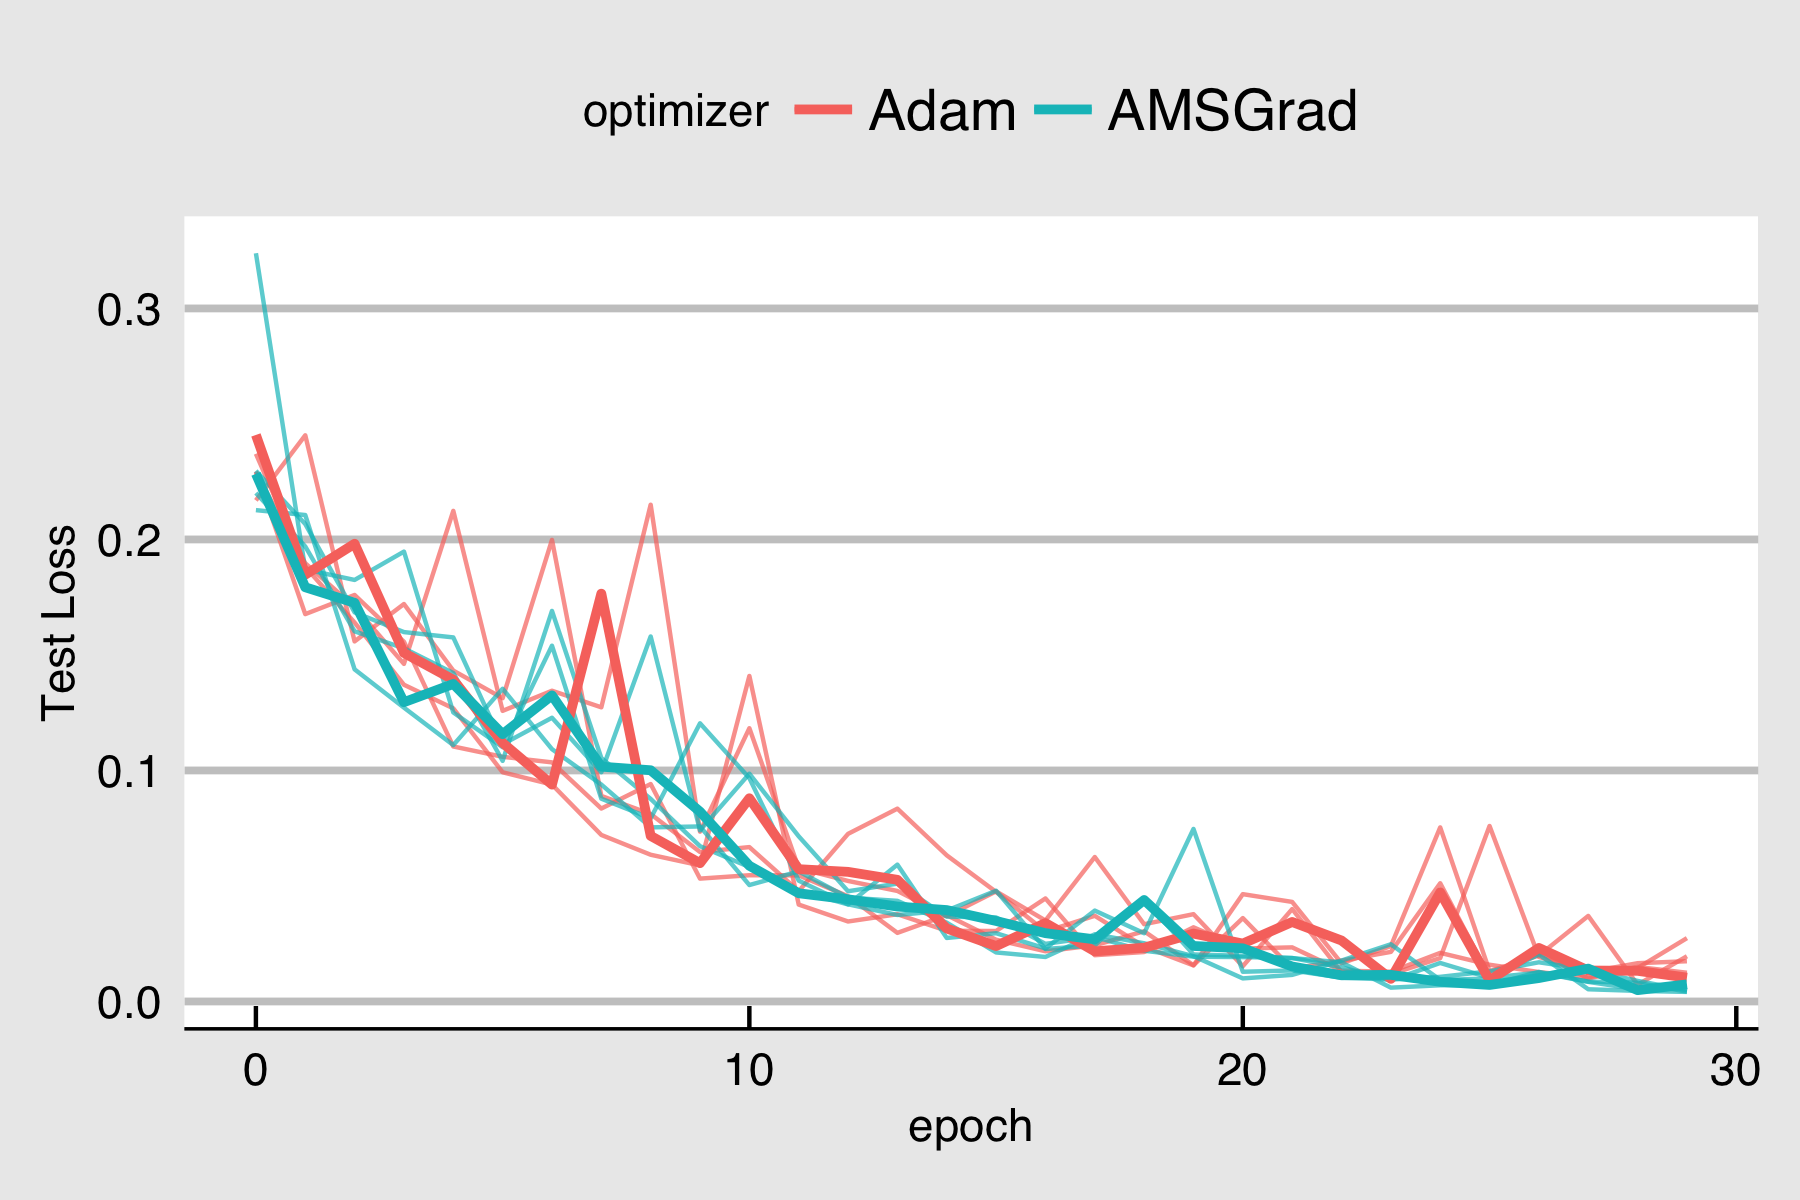
\includegraphics[width = 3.1in]{cifar_multi_testloss}} &
\subfloat{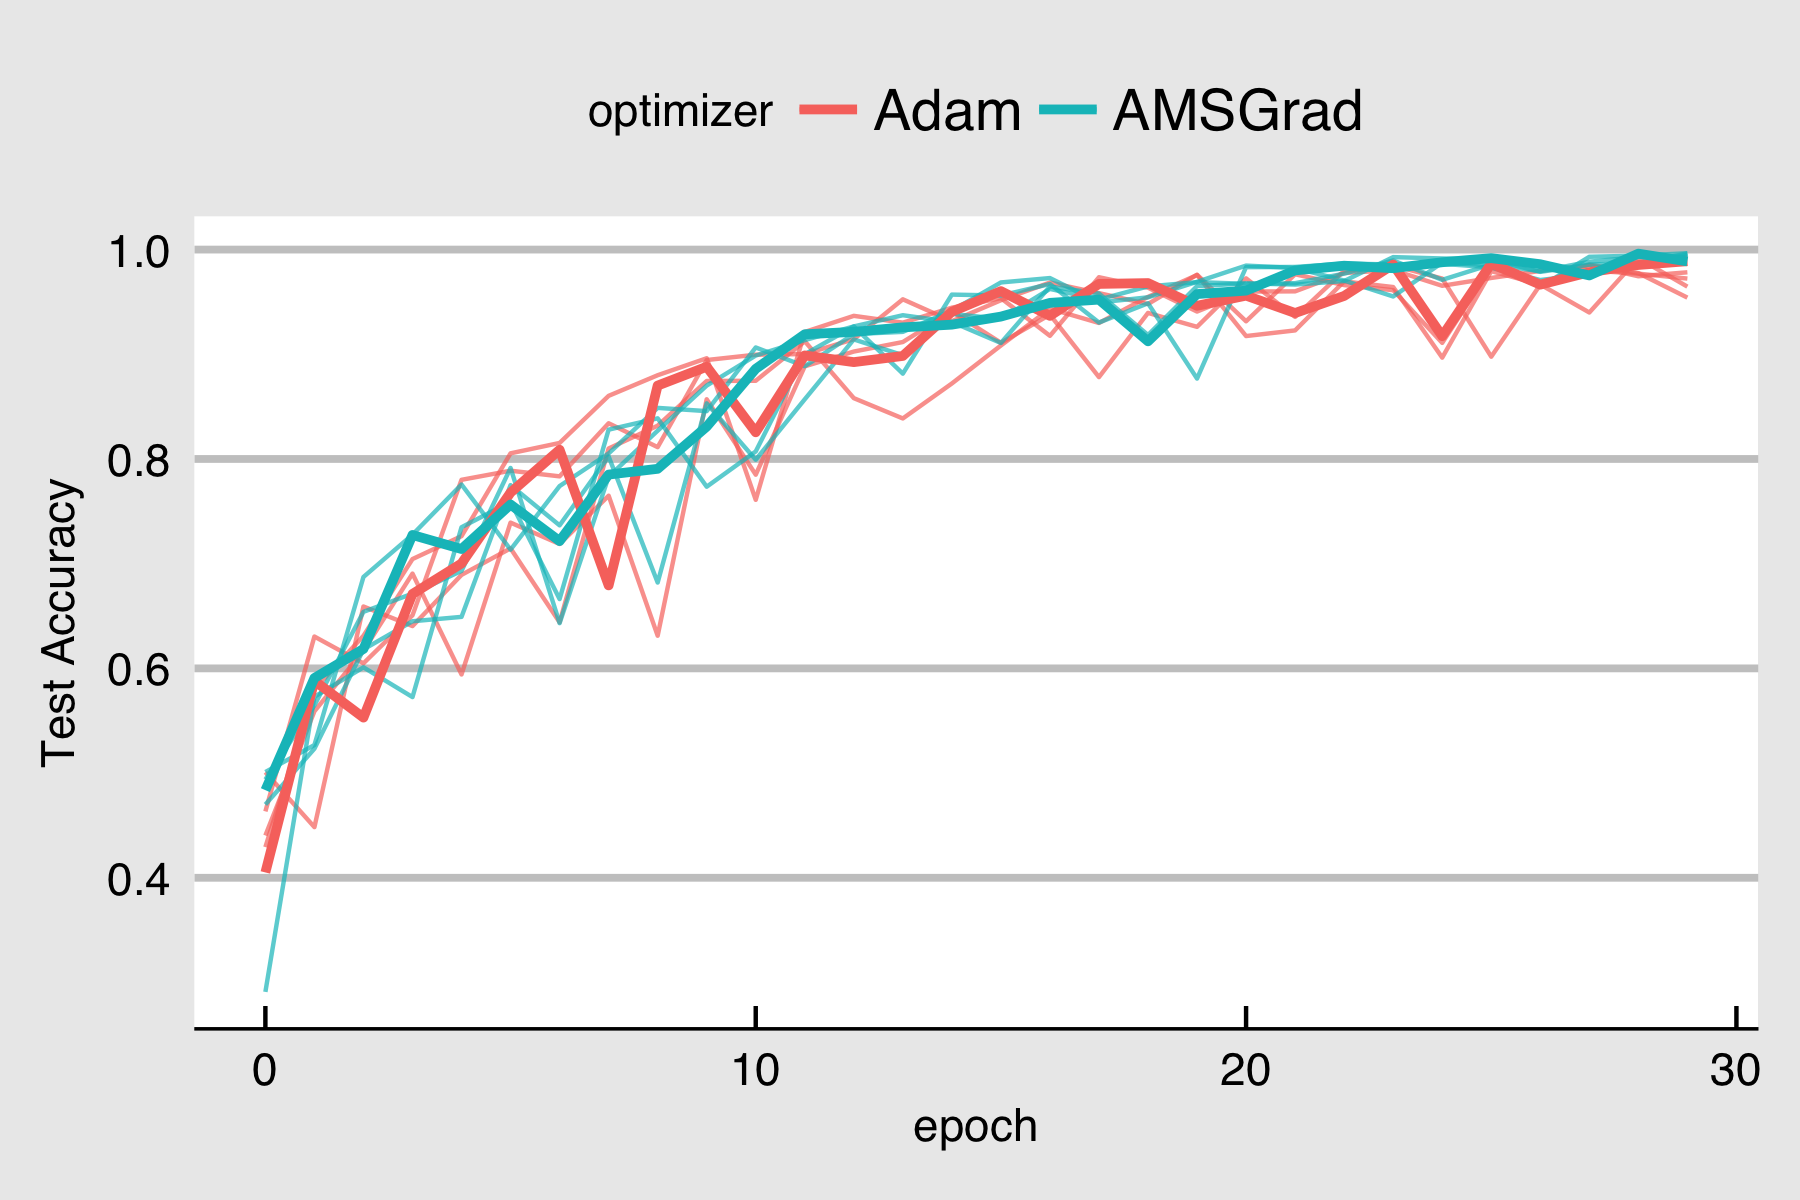
\includegraphics[width = 3.1in]{cifar_multi_test_acc}}
\end{tabular}
\caption{Training trajectories of Convolutional Neural Network model on CIFAR-10. The first run observed is in bold.\\
Top: training loss and accuracy. Bottom: test loss and accuracy.}
\end{figure*}

%%%%%%%%%%%%%%%%%%%%%%%%%%%%%%%%%%%%%%%%%%%%%%%%%%%%%%%%%%%%%%%%%%%%%%%%%%%%%%%%



\end{document}


